\documentclass[journal]{IEEEtran}
\usepackage{amsmath,amsfonts}
\usepackage{algorithmic}
\usepackage{array}
\usepackage[caption=false,font=normalsize,labelfont=sf,textfont=sf]{subfig}
\usepackage{textcomp}
\usepackage{stfloats}
\usepackage{url}
\usepackage{verbatim}
\usepackage{graphicx}
\usepackage{multirow}
\usepackage{algorithm}
\usepackage{cite}
\usepackage{algorithmic}
\usepackage{array}
\usepackage{booktabs}
\usepackage{longtable}
\usepackage{multicol, lipsum}
\usepackage{tabularx}
\usepackage{svg}
\usepackage{booktabs} 
\usepackage[colorlinks,linkcolor=blue]{hyperref}
% left fixed width:
\newcolumntype{L}[1]{>{\raggedright\arraybackslash}p{#1}}

% center fixed width:
\newcolumntype{C}[1]{>{\centering\arraybackslash}p{#1}}

% flush right fixed width:
\newcolumntype{R}[1]{>{\raggedleft\arraybackslash}p{#1}}
\hyphenation{op-tical net-works semi-conduc-tor IEEE-Xplore}
\def\BibTeX{{\rm B\kern-.05em{\sc i\kern-.025em b}\kern-.08em
		T\kern-.1667em\lower.7ex\hbox{E}\kern-.125emX}}
\usepackage{balance}

\newcommand{\R}{\mathbb{R}}
\begin{document}
	\title{Multi-Scale Grid Attention and Probabilistic Refinement for Accurate RoI-based Monocular 3D Object Detection}
	\author{Tingyu Zhang, Xinyu Yang, Zhigang Liang, Yanzhao Yang, and Jian Wang
		\thanks{Corresponding author: Jian Wang}
		\thanks{Tingyu Zhang, Zhigang Liang, Yanzhao Yang and Jian Wang are with College of Computer Science and Technology, Jilin University, Changchun, China}
		\thanks{Xinyu Yang is with Automotive safety and Simulation Test Department, China Automotive Innovation Corporation, Nanjing, China}}
	
	\markboth{}
	{Tingyu Zhang, Xinyu Yang, Zhigang Liang, Yanzhao Yang, Jian Wang:
		Multi-Scale Grid Attention and Probabilistic Refinement for Accurate ROI-based Monocular 3D Object Detection}
	
	\maketitle
	
	\begin{abstract}
		Monocular 3D object detection remains a challenging task due to the inherent limitations of single-view depth perception. While conventional methods treat all parts of the Region of Interest (RoI) uniformly, we argue that different RoI regions hold varying importance for accurate detection. This study introduces the Multi-Scale Grid Attention (MSGA) mechanism to investigate the significance of RoI regions at multiple scales. Furthermore, we propose a novel probabilistic post-processing method to enhance detection robustness by effectively utilizing the probabilistic properties of depth estimation during inference. Our approach achieves state-of-the-art performance on the KITTI and Waymo datasets, demonstrating significant improvements in detection accuracy and robustness.
	\end{abstract}
	
	\begin{IEEEkeywords}
		Camera, Intelligent vehicles, Monocular 3D object detection.
	\end{IEEEkeywords}
	
	
	\section{Introduction}
	\noindent\IEEEPARstart{M}{onocular} camera-based 3D object detection has become a significant research area in computer vision, with applications spanning autonomous driving, robotics, and augmented reality~\cite{tits survey}. Unlike conventional approaches dependent on depth sensors or multi-camera setups, monocular 3D object detection leverages the capabilities of a single camera to estimate the three-dimensional spatial information of objects within its field of view.
	
	The significance of monocular 3D object detection lies in its potential to provide depth perception using only the information captured by a single camera. This is particularly advantageous for real-world applications where cost, simplicity, and computational efficiency are essential considerations. Achieving accurate and robust 3D object detection from monocular images involves addressing complex challenges such as scale ambiguity, occlusions~\cite{tits shape aware}, and perspective distortions inherent to a single viewpoint.
	
	The absence of explicit depth information poses a significant challenge for monocular 3D detectors, leading to a considerable disparity compared to point cloud-based methods. To bridge this gap, certain approaches~\cite{gupnet, didm3d, neurocs} initially forecast multiple RoI candidates and subsequently generate predictions for each. 3D RoI-based methods, such as those discussed in~\cite{neurocs}, often depend on pre-trained 3D monocular detectors. In contrast, 2D RoI-based methods solely predict 2D bounding boxes, offering a lighter and more efficient alternative. Furthermore, given the real-time demands of 3D object detection, efficiency is paramount. Therefore, this paper exclusively focuses on 2D RoI-based methods.
	
	2D RoI-based methods~\cite{gupnet, didm3d} typically involve three key steps. Firstly, the RoI is partitioned into distinct segments, followed by the application of RoI feature extraction techniques (such as RoI Pooling~\cite{fast-rcnn}, RoI Warp~\cite{roi-warp}, and RoI Align~\cite{mask-rcnn}) to extract pertinent features. Secondly, the RoI is fed into a neural network to further refine these features and generate predictions for each region. Finally, the individual predictions are integrated to yield the final results.
	
	However, the second and third steps present certain challenges. In the second step, each partition of the RoI is treated equally in previous works, disregarding the varying importance of different RoI regions. For instance, empirically, information pertaining to the tire or license plate number holds more significance than that concerning the car body, and background regions should have less influence than foreground areas. Taking DID-M3D~\cite{didm3d} as an example, it predicts the depth to the object surface, referred to as visual depth, to decouple the depth. In the KITTI~\cite{kitti} dataset, the training data for the depth completion task and 3D object detection task do not entirely overlap, resulting in some images in KITTI 3D lacking ground truth visual depth. Therefore, DID-M3D introduces a depth completion network to generate a dense visual depth map. 
	
	We select images with depth labels and compare the ground truth with the depth map generated by the depth completion network. As depicted in Fig.~\ref{fig:depth_residual}, visual depth near the center of an object is more precise than at the edges. Taking the central visual depth of the RoI as the baseline, the distribution of visual depth in the RoI is imbalanced, as shown in Fig.~\ref{fig:visual_depth_offset}. Additionally, 2D RoIs are generated by the network, potentially resulting in incomplete object warping. To address these issues, we propose the MSGA module. Specifically, we enlarge the RoI by adding various pixels to its size, extract multi-scale features using a network, and apply a Grid Attention (GA) module to assess the importance of different regions and further adjust the RoI features.
	\begin{figure}[!t]
		\centering
		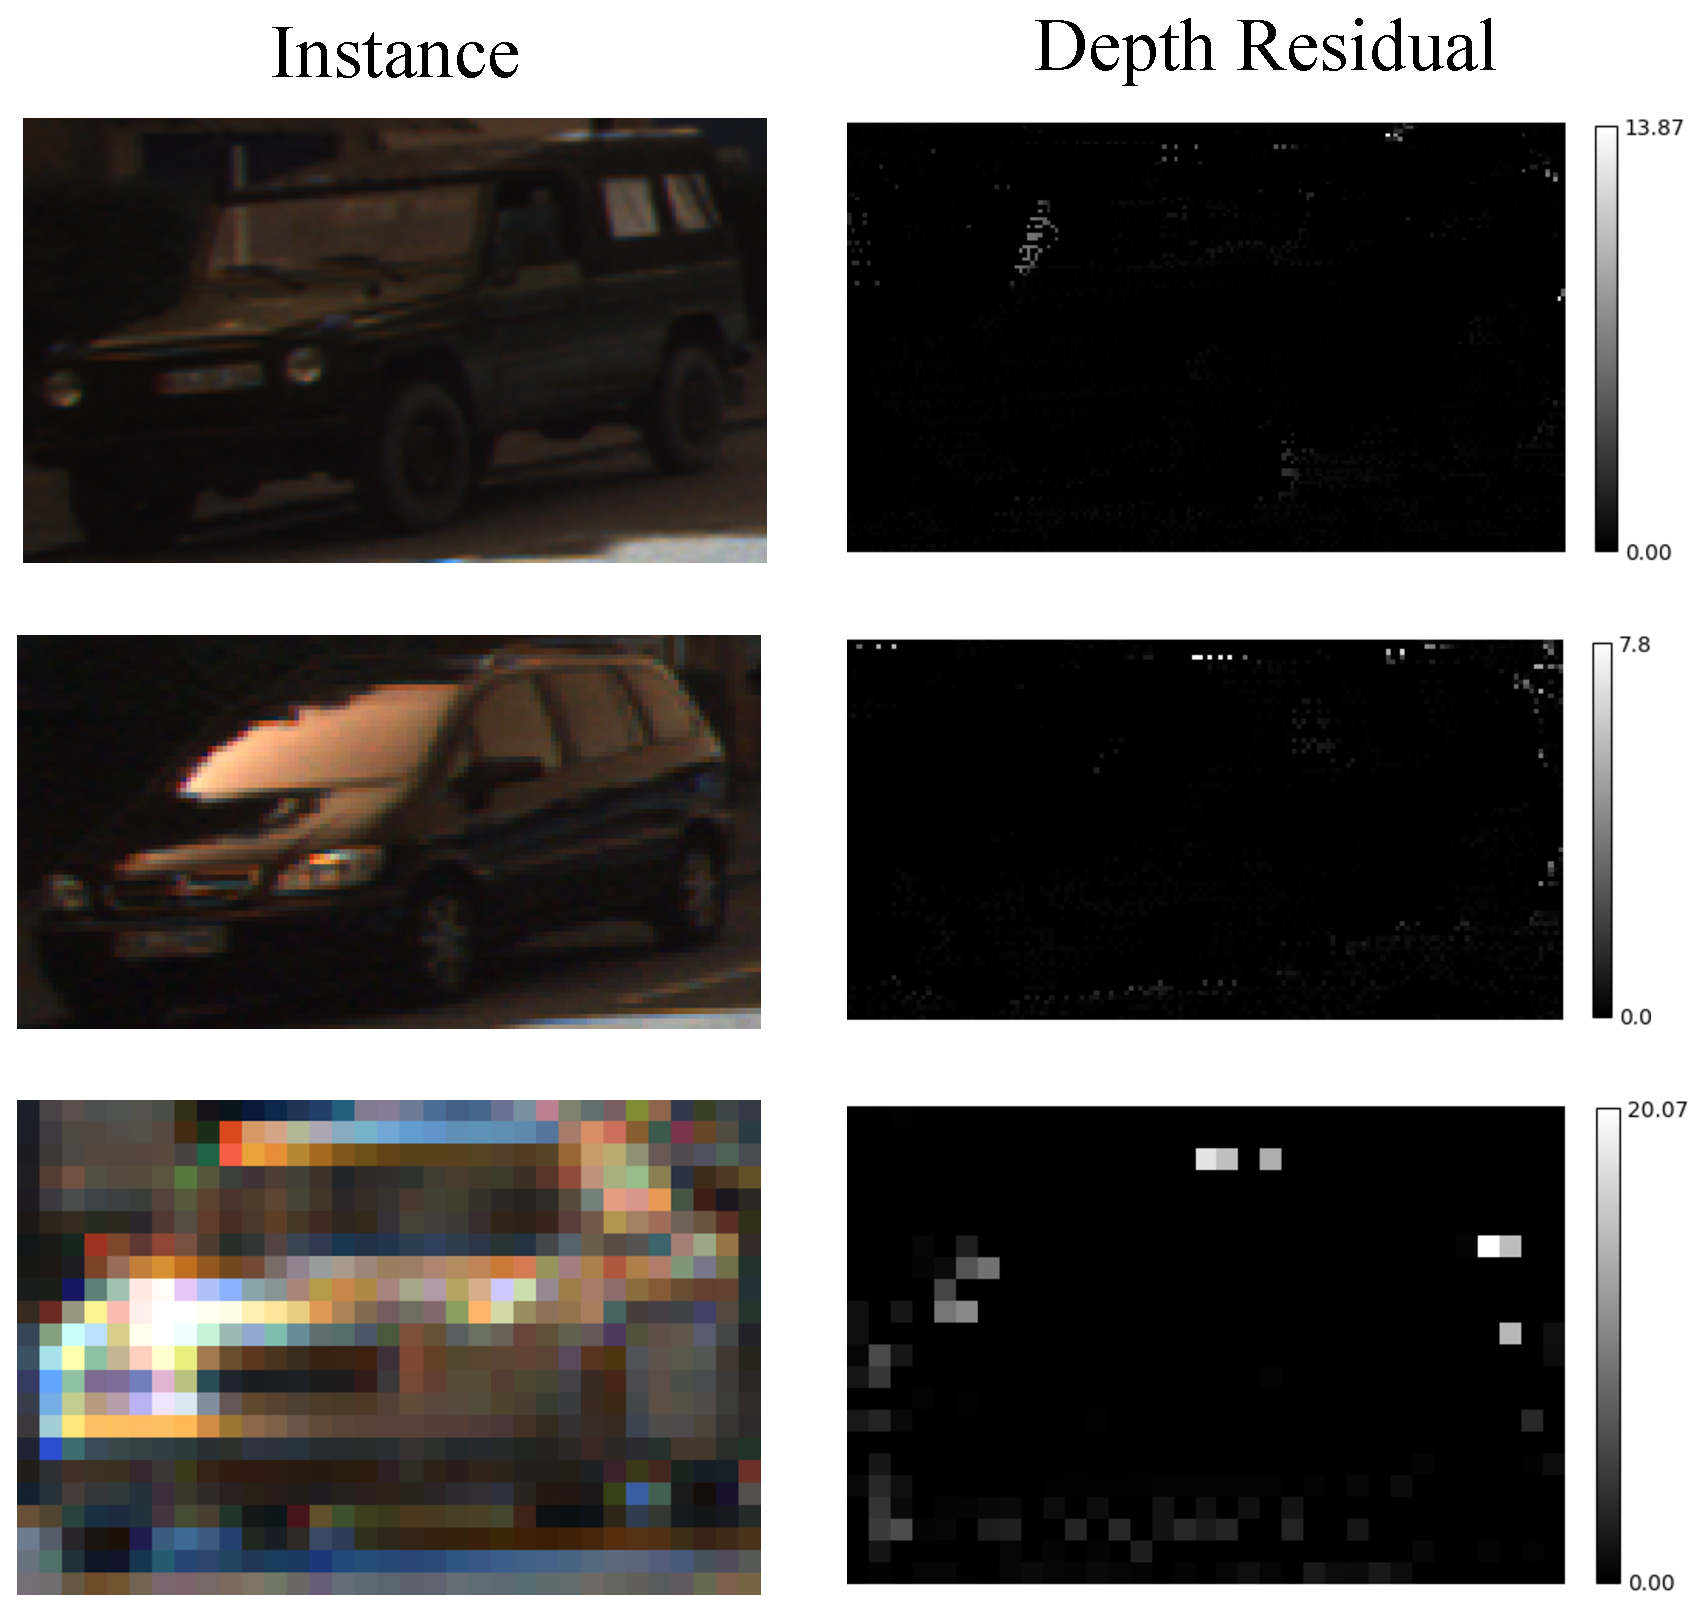
\includegraphics[width=1.0\linewidth]{depth_residual}
		\caption{Instance and its depth residual. The depth residual of an instance is computed by taking the absolute difference between the predicted depth generated by the depth completion network and the corresponding ground truth. The left column shows the raw image of the instance, while the right column illustrates the depth residual. Lighter colors in the latter column indicate higher depth residuals.}
		\label{fig:depth_residual}
	\end{figure}
	\begin{figure}[!t]
		\centering
		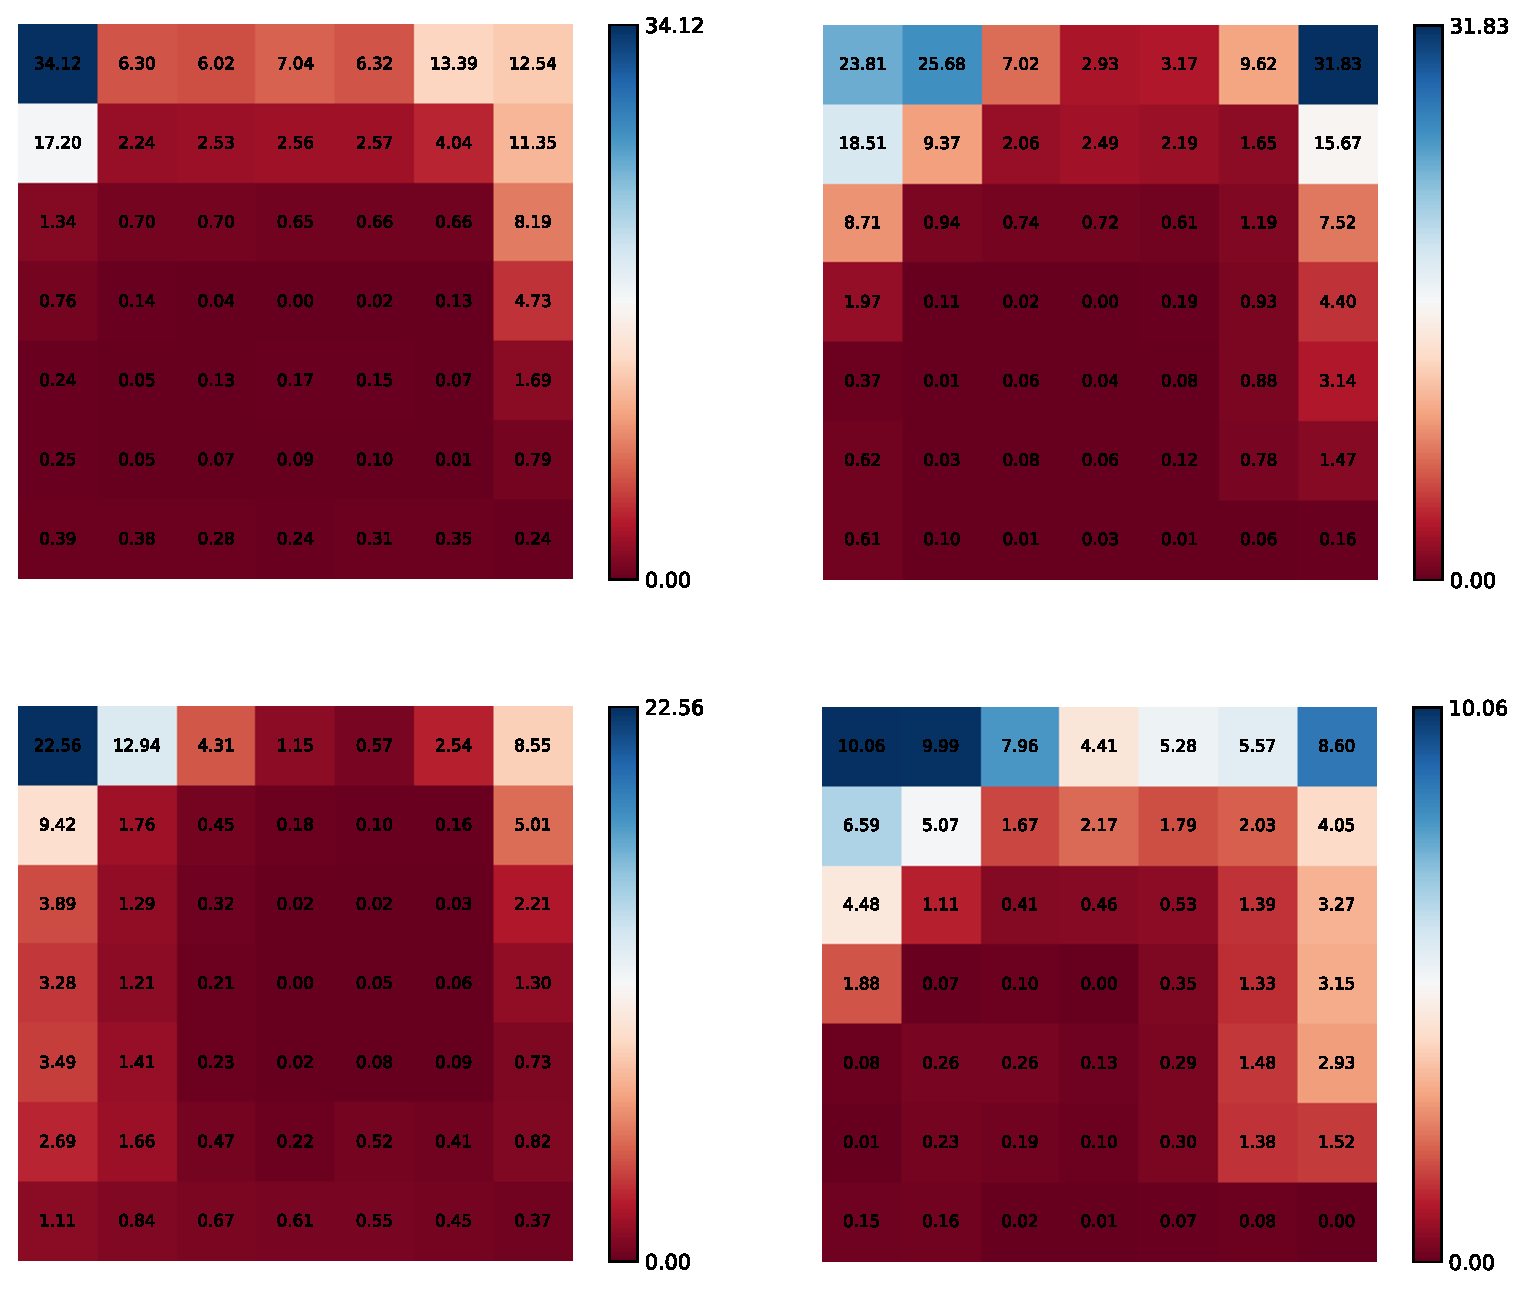
\includegraphics[width=1.0\linewidth]{visual_depth_offset.eps}
		\caption{Visual depth offset. The visual depth of the central grid within the RoI is considered the baseline, from which the offset to other grids is computed. This absolute offset is subsequently labeled for each grid.}
		\label{fig:visual_depth_offset}
	\end{figure}
	\begin{figure}[!t]
		\centering
		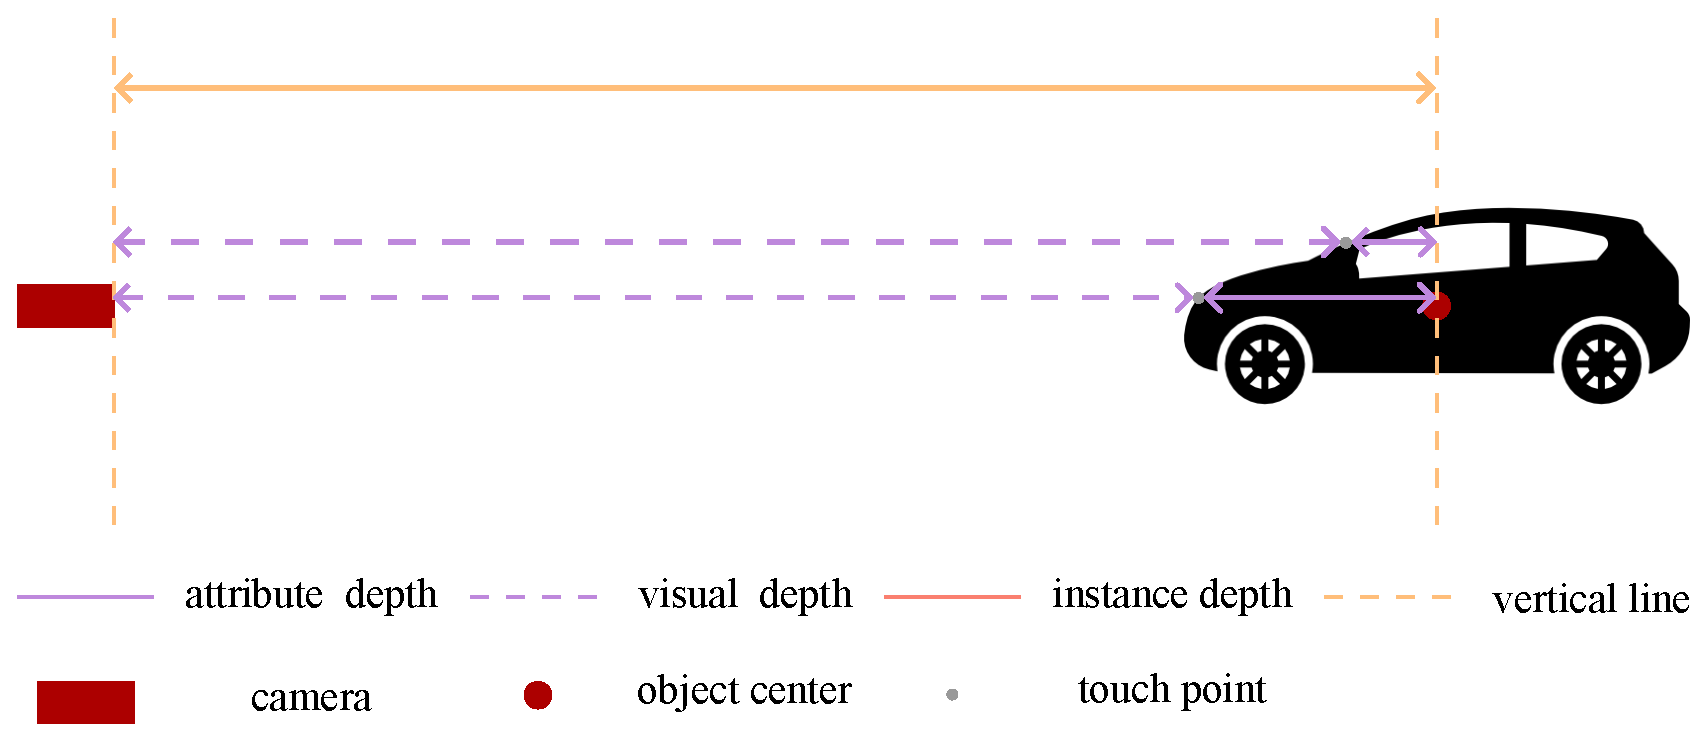
\includegraphics[width=1.0\linewidth]{decoupled_depth.eps}
		\caption{Decoupled depth. The instance depth is defined as the distance between the object center to the camera plane. And the visual depth is distance of object surface to the camera plane. The attribute depth is obtained by the minus of instance depth and visual depth.}
		\label{fig:decoupled depth}
	\end{figure}

	In the third step, the results are integrated to obtain the final outcomes. Previous approaches commonly employed simple averaging or weighted summation. While adequate for properties like dimensions and position, where each grid shares the same regression target, this method encounters challenges in depth estimation. In particular, depth is decomposed into visual depth and attribute depth~\cite{didm3d}, as illustrated in Fig.~\ref{fig:decoupled depth}. Each grid possesses distinct visual and attribute depths, leading to an imbalanced distribution that renders simple averaging suboptimal. Moreover, deriving the weights for weighted summation proves challenging. In our study, we adopt the assumption from previous research~\cite{gupnet, didm3d} that depth follows a certain distribution, leveraging this probability distribution in the post-processing phase. This approach enhances the integration process's rationality.
	
	
	In summary, our contributions can be outlined as follows:
	\begin{itemize}
		\item We meticulously explore the limitations of 2D RoI-based monocular 3D object detection, highlighting an inconsistency in the significance of RoI grids. We introduce the notion of varying importance among RoI grids and propose the utilization of Multi-Scale Grid Attention to address this issue.
		\item During the post-processing phase, we meticulously consider the assumed depth distribution, employing probabilistic methods for refinement.
		\item The experimental results underscore the superiority of our method compared to existing approaches on the KITTI and Waymo datasets.
	\end{itemize}
	
	\section{Related Work}
	\subsection{Monocular 3D Object Detection without RoI}
	Given the inherent challenges of directly estimating instance depth with a monocular camera due to its ill-posed nature, previous studies have sought to leverage these constraints effectively. Mousavian et al. \cite{geometry3d} introduced relationships between 2D and 3D bounding boxes to formulate a system of equations, incorporating specific priors such as driving direction to constrain the degrees of freedom. PGD \cite{pgd} and MonoPair \cite{monopair} investigate relationships among different instances, while DDMP-3D \cite{ddmp-3d} examines the relationships between neighboring pixels, using these constraints to refine box estimations. Recently, MonoCD~\cite{monocd} has fully exploited the geometric relationships among multiple depth cues to achieve complementary results.
	
	Some alternative methods \cite{m3d-rpn, d4lcn, monodtr} employ numerous anchors placed on the 3D plane and extract anchor features through projection. These approaches encounter common issues associated with anchor-based methods, including the proliferation of anchors and the nontrivial configuration of anchor hyperparameters.
	
	Due to the scale variance in the image plane and the notable success of LiDAR detectors, several methods endeavor to convert the 2D image plane into the 3D plane. OFT \cite{oft} and ImVoxelNet \cite{imvoxelnet} utilize the projection of predefined 3D voxels onto the image plane to populate the features of each voxel. CaDDN \cite{caddn} partitions the depth range into segments and predicts the probability for each segment, followed by the expansion of pixel features into frustum features. MonoDiscret~\cite{tits discrete depth} also discretizes the depth for more stable depth estimation. MonoNeRD \cite{mononerd} leverages 2D image features to generate NeRF-like 3D representations. Additionally, various pseudo-LiDAR methods \cite{color-embeded, mono-plidar, patchnet} integrate an independent depth completion network to generate a dense depth map, using the calibration matrix to derive the pseudo LiDAR. Subsequently, a LiDAR-based detector is employed to obtain the final results. Despite its success, DD3D \cite{dd3d} argues that pseudo LiDAR is unnecessary for detection. Instead, it employs a single model to predict depth and 3D bounding box simultaneously, obviating the need for an independent depth completion network.
	
	Monocular 3D object detection heavily relies on accurate depth estimation~\cite{monodle, tits monopixel, tits depth estimation}. Even slight errors in depth estimation can lead to objects being significantly offset from ground truth positions. To address this challenge, many methods aim to introduce additional supervision to constrain depth offsets. Key point estimation, as demonstrated in works such as Polygon~\cite{polygon}, is commonly employed because it imposes eight additional constraints on the model. Representative methods utilizing this approach include RTM3D~\cite{rtm3d}, SMOKE~\cite{smoke}, MonoDDE~\cite{monodde}, Monocon~\cite{monocon} and MonoAux~\cite{tits aux}, while MonOAPC~\cite{tits plane cons} paid more attention on occluded key points.
	
	Several methods utilize diverse strategies to improve performance. For instance, M3DSSD~\cite{m3dssd}, MonoPGC~\cite{monopgc}, CIE~\cite{cie}, MonoDETR~\cite{monodetr} and SSD-MonoDETR~\cite{ssd-monodetr} incorporate attention mechanisms to enhance results. MonoFlex~\cite{monoflex} specifically addresses truncated objects by predicting edge heatmaps. FD3D~\cite{fd3d} and ADD~\cite{add} implement auxiliary feature supervision to boost performance. OccupancyM3D~\cite{occupancym3d} introduces the concept of occupancy into monocular 3D object detection to improve its efficacy. Finally, MonoUNI~\cite{monouni} unifies monocular 3D detection for both vehicles and infrastructure through a proposed normalized depth approach.
	
	\subsection{Monocular 3D Object Detection with RoI}
	
	RoI-based object detection can be broadly categorized into 3D RoI-based and 2D RoI-based methods. 3D RoI-based approaches~\cite{neurocs, monoxiver} typically depend on a separately pretrained monocular 3D object detector to produce 3D proposals, a process that does not meet the real-time demands of autonomous driving. In contrast, 2D RoI-based methods~\cite{roi10d, didm3d, gupnet, gupnet++} share most of the network in both RoI generation and object detection, rendering them more efficient.
	
	In this study, our emphasis is on 2D RoI-based methods. Recognizing the challenges posed by RoI generation noise and the varying significance of RoI components, we introduce the MSGA module to effectively address these issues. Additionally, we introduce a novel probabilistic post-processing strategy to leverage the probabilistic assumptions inherent in depth estimation.
	\begin{figure*}[!t]
		\centering
		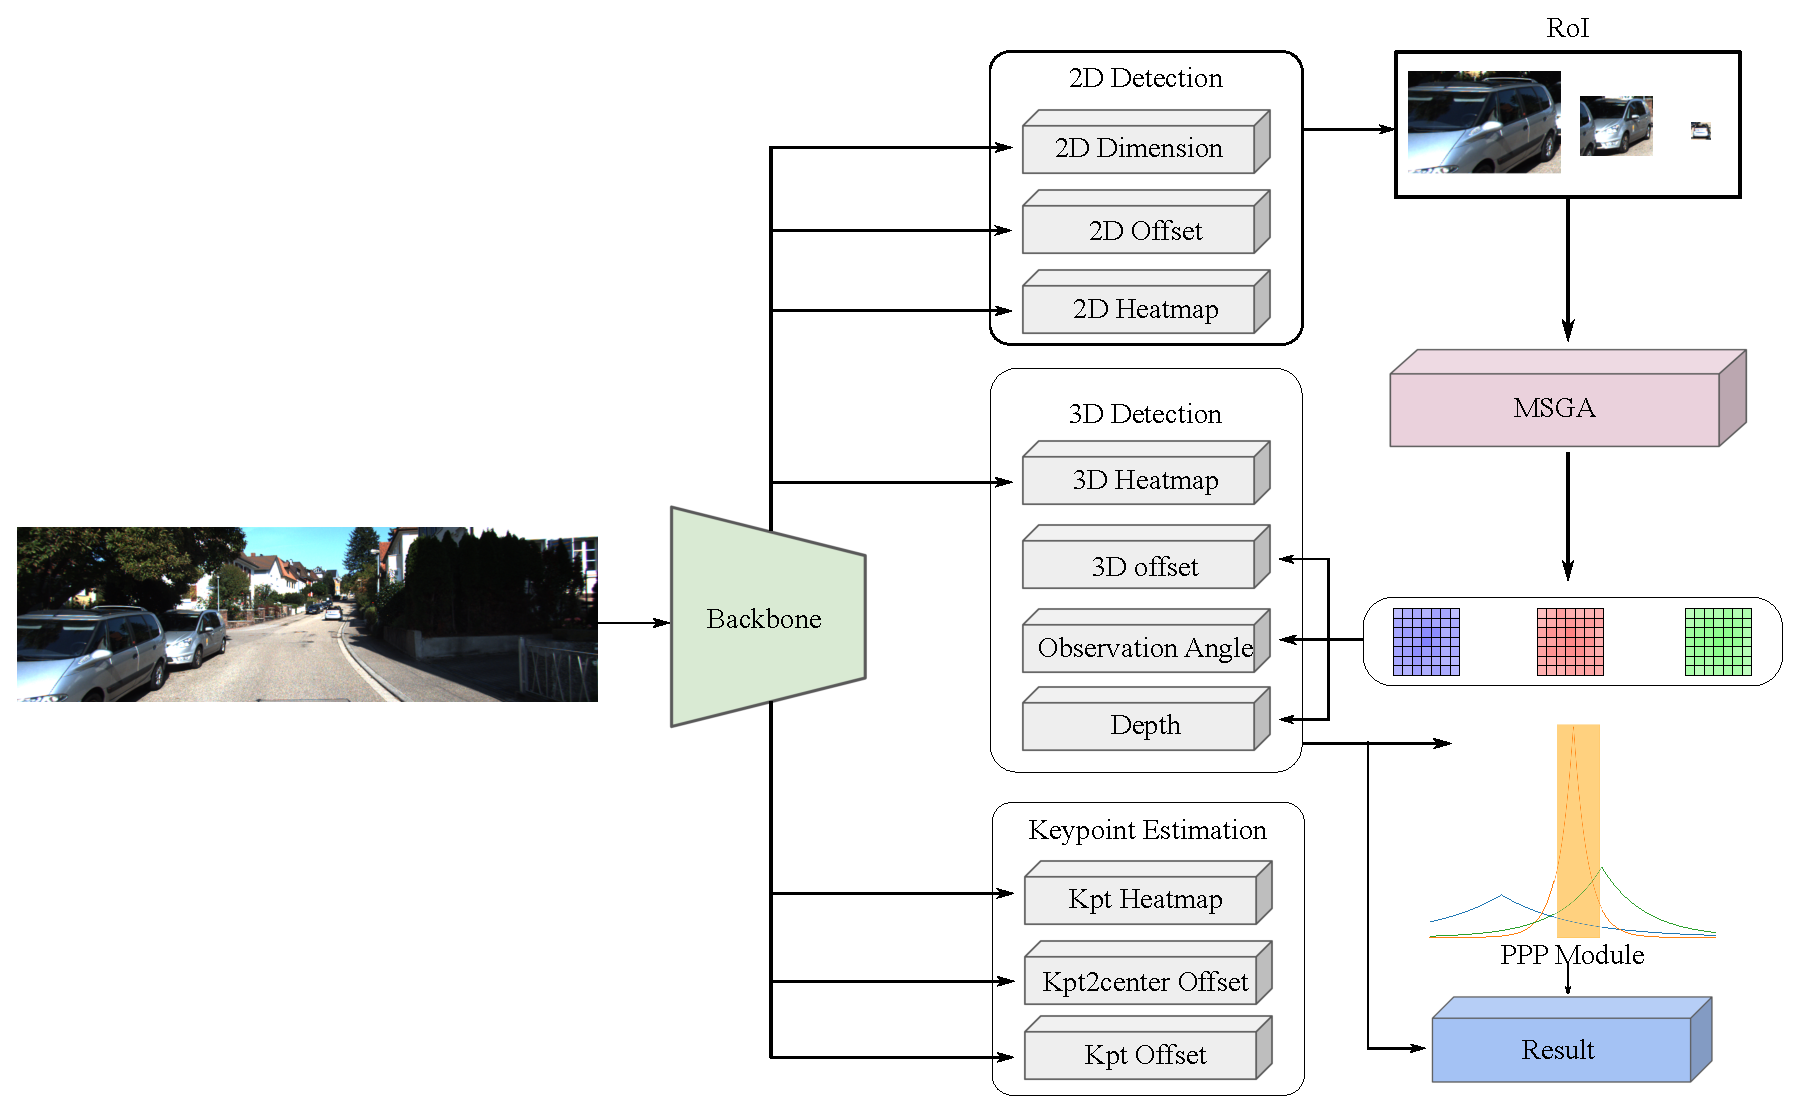
\includegraphics[width=1.0\linewidth]{overview.eps}
		\caption{Overview of our model. Initially, the input image undergoes processing through the backbone network to extract image features. These features are subsequently utilized for 2D detection, keypoint estimation, and 3D heatmap generation. Leveraging the results of 2D detection, the Region of Interest (RoI) features are directed to the Multi-Scale Grid Attention (MSGA) module for refinement. The enhanced RoI features are then employed to predict the 3D offset, observation angle, and depth. The depth estimation undergoes optimization via the Probabilistic Post-Processing (PPP) module. Finally, the results are decoded by both 3D properties and optimized depth.}
		\label{fig:overview}
	\end{figure*}
	
	\section{Method}\label{sec:method}
	\subsection{Problem Definition}
	In the domain of monocular 3D object detection, the primary input consists of the RGB image $I$. The main goal is to determine essential properties of the 3D bounding boxes, including the 3D center coordinates $x_c, y_c, z_c$, the 3D dimensions $l, w, h$ and the observation angle $\theta$, which is more related to image appearance than orientation angle~\cite{geometry3d}. A crucial element in this procedure is the projection matrix $P$, as described in Eq.~\eqref{eq:projection_matrix}.
	\begin{equation}
		P=\begin{pmatrix}f&0&c_u&-fb_x\\0&f&c_v&-fb_y\\0&0&1&-fb_z\end{pmatrix}
		\label{eq:projection_matrix}, 
	\end{equation}
	
	where $f$ denotes the focal length, while $c_u$ and $c_v$ denote the vertical and horizontal positions of the camera in the image, respectively. Furthermore, $b_x$, $b_y$ and $b_z$ indicate the baseline relative to the reference camera. 
	
	In a monocular setting, directly determining the 3D center position poses a significant challenge, mainly due to the considerable variability in 3D center scale. As a result, many studies opt to predict the projected 3D center on the image plane, denoted as $x_{ic}, y_{ic}$, along with the corresponding depth $d$. The recovery of the 3D bounding box center is then accomplished using Eq.~\eqref{eq:projection}.
	\begin{equation}
		dx_{2d} = Px_{3d}
		\label{eq:projection}, 
	\end{equation}
	
	where $P$ denotes the projection matrix, $x_{3d}$ represents the homogeneous 3D bounding box center $(x_c, y_c, z_c, 1)^T$, $x_{2d}$ signifies the homogeneous projected 3D center on the image plane $(x_{ic}, y_{ic}, 1)^T$, and $d$ denotes the depth of $x_{3d}$.
	
	\subsection{Overview}
	The schematic overview of our methodology is depicted in Fig.~\ref{fig:overview}. Initially, the provided image $I$ is processed through the image backbone, as discussed in Section~\ref{backbone}. Subsequently, a 2D detection head is employed to extract 2D properties, including the width and height of the bounding box, and to generate the heatmap for the projected 3D object center, as elaborated in Section~\ref{2d_detection_head}. Key point estimation, following the methodology of Monocon~\cite{monocon}, is incorporated into our approach. Utilizing the heatmap in conjunction with the predicted width and height, the 2D RoIs are determined. The RoIs are then input into the MSGA module to refine the features, as explained in Section~\ref{msga}. Employing the DID-M3D~\cite{didm3d} approach for each RoI grid, we predict both the visual depth and attribute depth, enabling subsequent prediction of 3D properties such as dimensions and observation angle. In the post-processing phase, we apply a novel depth integration strategy to consolidate RoI depths, taking into account the practical significance of probability distribution. This strategy is outlined in Section~\ref{post_processing}.
	
	\subsubsection{Image Backbone}\label{backbone}
	Given an input RGB image $I$ with dimensions $3 \times H \times W$, we utilize a feature backbone $f(\cdot; \Theta)$ to compute the feature map $F$ with dimensions $D \times h \times w$ as Eq.~\eqref{eq:backbone}.
	\begin{equation}
		F = f(I;\Theta)
		\label{eq:backbone}, 
	\end{equation}
	
	where $\Theta$ represents all learnable parameters, $D$ denotes the output feature map dimension (e.g., $D=512$), and $h$ and $w$ are determined by the overall subsampling rate $s$ in the backbone (e.g., $s=4$). We employ the DLA-34~\cite{dla} network as our chosen backbone.
	
	\subsubsection{2D Detection Head}\label{2d_detection_head}
	Utilizing the output feature map $F$ from the backbone as input, we route it through three detection heads. Each detection head comprises a series of operations: a 2D convolution, Rectified Linear Unit (ReLU) activation function, followed by another 2D convolution. Specifically, the first detection head is responsible for predicting the heatmap $H$ indicating the projected 3D object center. The process of heatmap generation follows the methodology outlined in CenterNet~\cite{centernet}. The second detection head focuses on predicting the offsets $\Delta x$ and $\Delta y$ between the projected 3D object center and the center of the 2D bounding box. Finally, the third detection head is tasked with predicting the width $w_{2d}$ and height $h_{2d}$ of the 2D bounding box.
	
	\subsubsection{Multi-Scale Grid Attention Module}\label{msga}
	During the training phase, we utilize the ground truth projected 3D object center $(x_{c_{gt}}, y_{c_{gt}})$, predicted offsets $\Delta x$ and $\Delta y$, as well as the predicted width $w_{2d}$ and height $h_{2d}$ of the 2D bounding box to compute the RoI using Eq.~\eqref{eq:RoI_generation}. Each RoI is defined by its top-left and bottom-right boundary points.
	\begin{equation}
		\begin{aligned}
			RoI =& (x_{c_{gt}}-w_{2d}/2, y_{c_{gt}}-h_{2d}/2, \\
			&x_{c_{gt}}+w_{2d}/2, y_{c_{gt}}+h_{2d}/2)
			\label{eq:RoI_generation}.
		\end{aligned}
	\end{equation}
	
	During the inference phase, we select the top 50 positions from the heatmap to represent the predicted projected 3D object center. Subsequently, we combine the predicted offset and 2D dimensions to generate the RoI.
	\begin{figure*}
		\centering
		\includegraphics[width=1.0\linewidth]{Multi-Scale-Grid-Attention.eps}
		\caption{Multi-Scale Grid Attention Module. We use three scale to generate the RoI, the RoI feature is obtained by RoI Align. We use 1D convolutional network to generate the attention map of RoI grid. Then we multiply the attention map and the RoI feature, fed to residual summation for the merged feature. The final feature is integrated by the multi-scale merged feature.} 
		\label{fig:multi-scale-grid-attention}
	\end{figure*}
	
	Adjacent background information plays a crucial role in distinguishing foreground instances~\cite{pyramid-rcnn}, particularly when the predicted RoI may not accurately encapsulate the object. Similarly, in point cloud-based 3D object detection, such as Pyramid-RCNN~\cite{pyramid-rcnn}, 3D RoIs encounter analogous challenges. To address this issue, enlarging the RoI is a common strategy. In Pyramid RCNN, the RoI is expanded proportionally based on the original RoI. In 3D dimensions, scale remains constant, implying consistent object dimensions irrespective of distance. In contrast, in the image plane, scale varies with distance. Proportional enlargement may not be optimal, potentially introducing excessive background pixels for nearby objects. Thus, we adopt a fixed number of pixels enlargement strategy for the RoI. Determining the required pixels for RoIs with different sizes and varying accuracies of 2D bounding box prediction is challenging. 
	
	To overcome this challenge, we propose a Multi-Scale configuration, illustrated in Fig~\ref{fig:multi-scale-grid-attention}. Initially, the original RoI is cropped by the predicted 2D bounding box. We uniformly increase the width and height of the 2D bounding box by 5 and 15 pixels, respectively, to create the enlarged RoI. Subsequently, RoI Align~\cite{mask-rcnn} is applied to generate $7\times 7$ RoI features. A $1\times 1$ convolution and sigmoid function are then applied to generate the attention map for each grid. The RoI feature is multiplied by the attention map, and the result is added to the RoI feature to obtain the merged feature. Finally, the multi-scale merged features are concatenated to form the final feature.
	
	The MSGA module consists of two key components: the multi-scale RoI feature and the Grid Attention mechanism. The advantages of employing the multi-scale RoI feature are elucidated as follows:
	\begin{itemize}
		\item Enhanced inclusion of foreground pixels: multi-scale features mitigate errors in 2D bounding box predictions, improving the likelihood of encompassing whole foreground pixels of the predicted object.
		\item Improved background information utilization: by incorporating adjacent background pixels, multi-scale features enable better extraction of information from the background region.
	\end{itemize}
	
	The advantages of the Grid Attention mechanism are summarized as follows:
	\begin{itemize}
		\item Discriminative pixel attention: grid attention enables the model to discern between background and foreground pixels, prioritizing for more accurate training. This discrimination enhances the model's ability to focus on relevant visual elements.
		\item Importance discrimination among foreground pixels: grid attention further discriminates among foreground pixels, assigning higher importance to specific elements. For instance, identifying features like a vehicle's license plate, which serves as a distinctive identifier, is prioritized.
	\end{itemize}
	
	\subsubsection{3D Detection Head}\label{3d_detection_head}
	
	For each set of RoI features, we employ seven distinct detection heads to predict various properties. These include the 3D dimensions offset, denoted as $dim_{3d}$, in comparison to the mean size of each class; the offset $offset_{3d}$ representing the quantization error between the projected 3D object center and the corresponding pixel; the visual depth $d_{vis}$ and its associated uncertainty $\sigma_{vis}$; the attribute depth $d_{att}$ and its corresponding uncertainty $\sigma_{att}$; and the observation angle $\theta$.
	
	The detection heads responsible for predicting $dim_{3d}$, $offset_{3d}$, and $\theta$ consist of a sequence comprising a 2D convolution layer followed by batch normalization, Rectified Linear Unit, and another 2D convolution layer. Conversely, the detection heads tasked with predicting $d_{vis}$, $\sigma_{vis}$, $d_{att}$, and $\sigma_{att}$ are composed of a 2D convolution layer, LeakyReLU activation function~\cite{leaky-relu}, and another 2D convolution layer.
	
	\subsubsection{Keypoint Estimation}
	For keypoint estimation, we adopt the approach proposed by Monocon~\cite{monocon}. Specifically, we estimate the keypoint heatmap $H_k \in \R^{9\times w \times h}$ to predict the projected positions of the 8 corners and the center of the 2D bounding box. Estimating $H_k$ involves a series of operations: a 2D convolution, ReLU activation, and another 2D convolution. Additionally, we predict the offsets $(\Delta k2c_x, \Delta k2c_y)$between each keypoint and the projected 3D object's center pixels, as well as the quantization error $(\Delta kx, \Delta ky)$ resulting from rounding off the keypoint positions. These components are determined through a sequence of operations: a 2D convolution, batch normalization, ReLU activation, and another 2D convolution. It's important to note that keypoint estimation is employed solely during training to provide supplementary supervision and is not utilized during inference.
	
	\subsubsection{Loss Functions}
	\paragraph{2D Heatmap} Our loss function follows the methodology outlined in CenterNet~\cite{centernet}. To guarantee a bounding box overlap of at least 0.7 IoU with the ground truth, we calculate the radius accordingly. Specifically for $H$, we utilize a modified focal loss, defined as Eq.~\eqref{eq:heatmap loss}.
	
	\begin{equation}
		\begin{split}
			L_{heat}=\frac{-1}N\sum_{H}\begin{cases}(1-H)^\alpha\log(H)&\text{if }\hat{H}=1\\(1-\hat{H})^\beta({H})^\alpha \\ \log(1-{H}) &\text{otherwise}\end{cases}, 
			\label{eq:heatmap loss}
		\end{split}
	\end{equation}
	
	where $\hat{H}$ denotes the target heatmap, with $N$ representing the number of keypoints in the image. For our experiments, we set the hyper-parameters $\alpha$ and $\beta$ for the focal loss to 2 and 4, respectively.
	
	\paragraph{2D Box} 
	For the 2D bounding boxes, we predict the offsets between the peak in the 2D heatmap $H$ and the center of the 2D bounding box, denoted as $\Delta x_{2d}$ and $\Delta y_{2d}$, along with the sizes of the bounding box, represented by $h_{2d}$ and $w_{2d}$. These values are determined using the L1 loss, as formulated in Eq.~\eqref{eq:2d box loss}.
	\begin{equation}
		L_{box_{2d}} = \sum_{o\in \{\Delta x_{2d}, \Delta y_{2d}, w_{2d}, h_{2d}\}}\lvert o - \hat{o} \rvert
		\label{eq:2d box loss}, 
	\end{equation}
	
	where $o$ denotes the predicted value and $\hat{o}$ denotes the regression target.
	\paragraph{3D Box}
	For 3D box, we need to regress the offset between the peak in 2D heatmap and the projected 3D object center $\Delta x_{3d}, \Delta y_{3d}$, along with the offset of ground truth dimensions and the averaged dimensions $\Delta l_{3d}, \Delta w_{3d}, \Delta h_{3d}$. They are all calculated by the L1 loss, which is formulated as Eq.~\eqref{eq:3d box loss}.
	\begin{equation} 
		L_{box_{3d}} = \sum_{o\in \{\Delta{x_{3d}}, \Delta{y_{3d}}, \Delta l_{3d}, \Delta w_{3d}, \Delta h_{3d}\}}\lvert o - \hat{o} \rvert
		\label{eq:3d box loss}.
	\end{equation}
	
	\paragraph{Depth}
	For depth estimation, we make the assumption that the depth follows the Laplace distribution~\cite{didm3d}, and use Eq.~\eqref{eq:depth loss} to calculate different depth and its uncertainty. 
	\begin{equation} 
		L_{depth} = \sum_{*\in \{vis, att, ins\}} \frac{\sqrt{2}}{e^{\frac{u_*}{2}}} \times \lvert d_* - \hat{d_*} \rvert + \frac{u_*}{2}
		\label{eq:depth loss}, 
	\end{equation}
	
	where $d_{vis}$, $d_{att}$, and $d_{ins}$ represent the visual depth, attribute depth, and instance depth, respectively, while $u_{vis}$, $u_{att}$, and $u_{ins}$ denote the uncertainty associated with each depth. The symbol $\hat{d_*}$ denotes the regression target. It's essential to clarify that our network predicts only the visual depth and attribute depth, with the instance depth computed as the sum of these two. Additionally, we calculate the instance depth uncertainty using Eq.~\eqref{eq:instance uncertainty}.
	\begin{equation} 
		u_{ins} = log(e^{u_{vis}} + e^{u_{att}})
		\label{eq:instance uncertainty}.
	\end{equation}
	\paragraph{Orientation Angle}
	We employ the Multi-bin loss~\cite{geometry3d} for the observation angle. Specifically, we partition $2 \pi$ into 12 bins, and the network generates the classification vector $\theta_{cls}$ to identify the bin in which the angle lies, along with the offset $\theta_{reg}$ between the bin center and the ground truth angle. The cross-entropy loss is utilized for $\theta_{cls}$, as formulated in Eq.~\eqref{eq:angle loss}.
	\begin{equation} 
		L_{angle_{cls}} = -\sum_{i=1}^{12} y_{i}\log(p_{i}), 
		\label{eq:angle loss}
	\end{equation}
	
	where $y_i$ as the indicator for the $i$th bin, where it equals 1 if the angle falls within the bin, and 0 otherwise. $p_i$ represents the predicted probability of the $i$th bin. As for $\theta_{reg}$, we employ the L1 loss, as formulated in Eq.~\eqref{eq:angle reg loss}.
	
	
	\begin{equation} 
		L_{angle_{reg}} = \lvert \theta_{reg} - \hat{\theta_{reg}} \rvert, 
		\label{eq:angle reg loss}
	\end{equation}
	
	where $\hat{\theta_{reg}}$ is the regression target.
	
	\paragraph{Keypoints}
	We incorporate an auxiliary keypoint loss inspired by Monocon~\cite{monocon}. To generate the keypoint heatmap $H_k \in \R^{9 \times w \times h}$, we project the eight corners onto the image plane and use the center of 2D bounding box, thus representing nine keypoints. The loss function mirrors that of the 2D heatmap, albeit with a looser IoU threshold of 0.3, as adopted in Monocon~\cite{monocon}. This loss function is detailed in Eq.~\eqref{eq:keypoint heatmap loss}.
	\begin{equation}
		\begin{split}
			L_{H_k}=\frac{-1}N\sum_{H_k}\begin{cases}(1-H_k)^\alpha\log(H_k)&\text{if }\hat{H_k}=1\\(1-\hat{H_k})^\beta({H_k})^\alpha \\ \log(1-{H_k}) &\text{otherwise}\end{cases}.
			\label{eq:keypoint heatmap loss}
		\end{split}
	\end{equation}
	
	In addition to the keypoint heatmap, we also predict the offset between each keypoint and the projected 3D object center pixel, denoted as $\Delta k2c_x$ and $\Delta k2c_y$, along with the offset between the peak in the keypoint heatmap and the keypoint position, represented as $\Delta kx$ and $\Delta ky$. These offsets are all calculated using the L1 loss, as formulated in Eq.~\eqref{eq:keypoint loss}.
	\begin{equation}
		L_{keypoint} = \sum_{i=1}^{9}\sum_{o\in \{\Delta k2c_x, \Delta k2c_y, \Delta kx, \Delta ky\}}\lvert o^i - \hat{o^i} \rvert, 
		\label{eq:keypoint loss}
	\end{equation}
	
	where $o^i$ denotes the prediction of the $i$-th keypoint, while $\hat{o^i}$ signifies the target corresponding to the $i$-th keypoint.
	
	The total loss is computed as the summation of the aforementioned losses, as defined in Eq. \eqref{eq:total loss}.
	\begin{equation}
		\begin{aligned}
			L_{total} =& \lambda_{heat}L_{heat} + \lambda_{box_{2d}}L_{box_{2d}} + \lambda_{box_{3d}}L_{box_{3d}}\\ 
			&+ L_{depth} +\lambda_{angle}(L_{angle_{cls}} + L_{angle_{reg}})\\ 
			&+ \lambda_{H_k}L_{H_k} + \lambda_{keypoint}L_{keypoint}, 
			\label{eq:total loss}
		\end{aligned}
	\end{equation}
	
	where $\lambda_*$ is the weight of each loss, is dynamically adjusted through hierarchical task learning, as proposed by GUPNet~\cite{gupnet}. Details of this adaptation process will be elucidated in Section~\ref{imple}.
	
	
	
	\begin{figure}[!t]
		\centering
		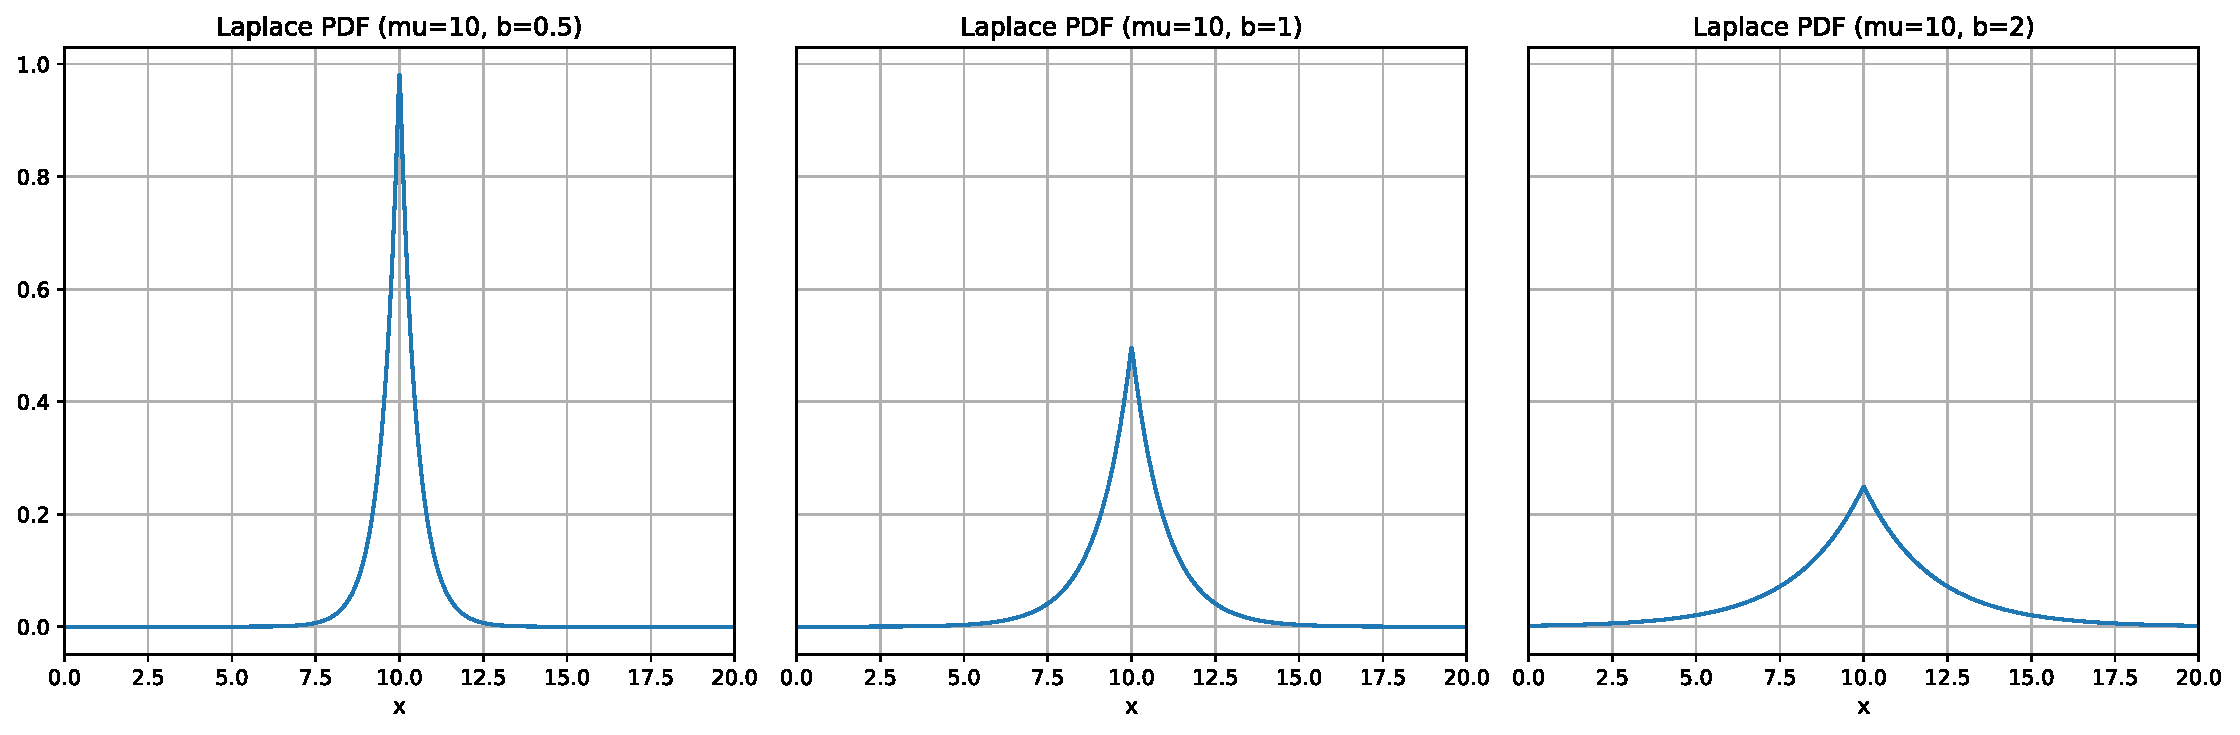
\includegraphics[width=1.0\linewidth]{laplace_distribution.eps}
		\caption{Laplace Probability Density Function. Left distribution means $\mu=10, b=0.5$. Middle distribution means $\mu=10, b=1$. Right distribution means $\mu=10, b=2$.}
		\label{fig:laplace distribution}
	\end{figure}
	\subsection{Probabilistic Post Processing}\label{post_processing}
	Previous studies have assumed that depth adheres to the Laplace distribution. The Probability Density Function (PDF) of the Laplace distribution is defined as shown in Eq. \eqref{eq:laplace pdf}. 
	\begin{equation}
		f(x|\mu,b)=\frac1{2b}\exp\left(-\frac{|x-\mu|}b\right), 
		\label{eq:laplace pdf}
	\end{equation}
	
	where $\mu$ represents the positional parameter, and $b$ represents the scale parameter. As illustrated in Fig.~\ref{fig:laplace distribution}, decreasing $b$ sharpens the PDF curve, while increasing it flattens the curve. In our work, the predicted uncertainty is the standard derivation of the Laplace distribution which is directly proportional to $b$. When uncertainty is smaller, the depth distribution becomes more concentrated, whereas larger uncertainty results in a more dispersed depth distribution.
	
	Previous methods~\cite{didm3d, gupnet} have utilized the standard deviation $\sigma$ which is adhere to the predicted uncertainty to assess the accuracy of depth estimation, employing $e^{-\sigma}$ to gauge the confidence level of the estimation. However, the rationale behind importance estimation lacks a solid theoretical foundation. In GUPNet \cite{gupnet}, it is stated that their objective is merely to normalize the value between 0 and 1. In this study, we introduced the Probabilistic Post-Processing (PPP) module to incorporate probabilistic distributions into our method.
	
	Based on fundamental probabilistic principles, the probability of a variable lying within the narrow range $[x-\delta, x+\delta]$ can be computed by calculating the area bounded by the PDF curve and the axis within that range. This computation can be performed using a definite integral or by subtracting the Cumulative Density Function (CDF). The CDF for the Laplace distribution is defined as shown in Eq.~\eqref{eq:laplace cdf}.
	\begin{equation}\begin{aligned}
			F(x)& =\int_{-\infty}^xf(u)\mathrm{d}u  \\
			&=\begin{cases}\frac12\exp\left(-\frac{\mu-x}b\right)&\mathrm{if~}x<\mu\\
				\\1-\frac12\exp\left(-\frac{x-\mu}b\right)&\mathrm{if~}x\geq\mu\end{cases} \\
			&=0.5\left[1+\mathrm{sgn}(x-\mu)\left(1-\exp(-|x-\mu|/b)\right)\right], 
			\label{eq:laplace cdf}
	\end{aligned}\end{equation}
	\begin{figure}[!t]
		\centering
		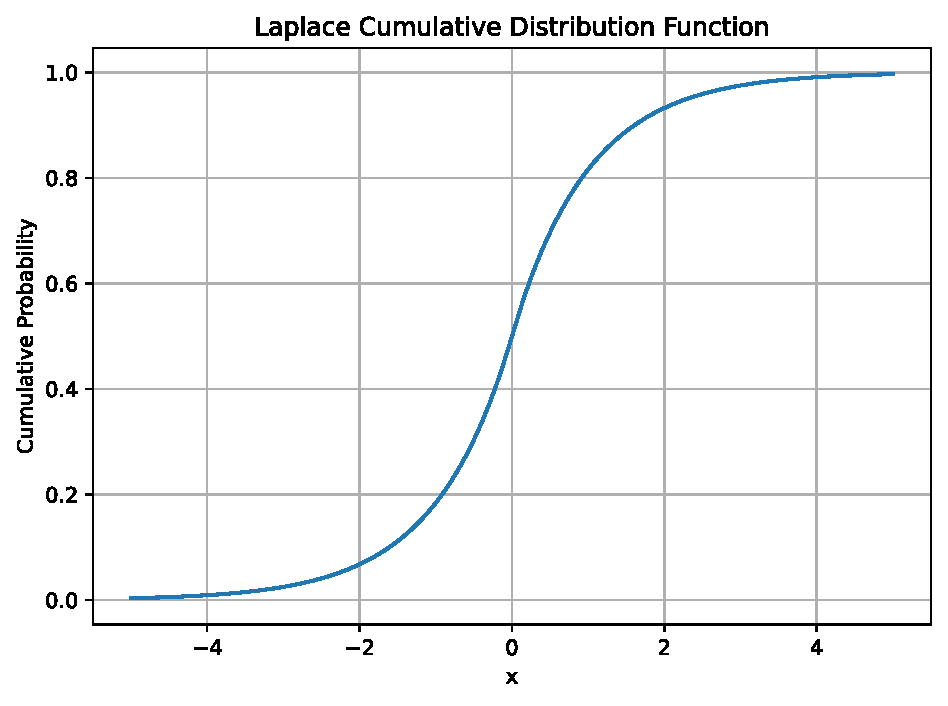
\includegraphics[width=1.0\linewidth]{laplace_cdf.eps}
		\caption{Laplace Cumulative Density Function.}
		\label{fig:laplace distribution cdf}
	\end{figure}
	
	where $\mathrm{sgn}(\cdot)$ denotes the sign function, while $F(x)$ represents the probability of a sample lying within the range $(-\infty, x]$. The CDF curve is illustrated in Fig.~\ref{fig:laplace distribution cdf}.
	
	In this work, we use the idea of maximum likelihood function. As above said, we can calculate the probability of the variable locating in the range $[x-\delta, x+\delta]$ by $F(x+\delta)-F(x-\delta)$. And we define the likelihood function as Eq.~\eqref{eq:likelihood function}. 
	\begin{equation}
		L(x) = \sum_{1}^{49} F(x+\delta)-F(x-\delta).
		\label{eq:likelihood function}
	\end{equation}
	
	\begin{figure}[!ht]
		\centering
		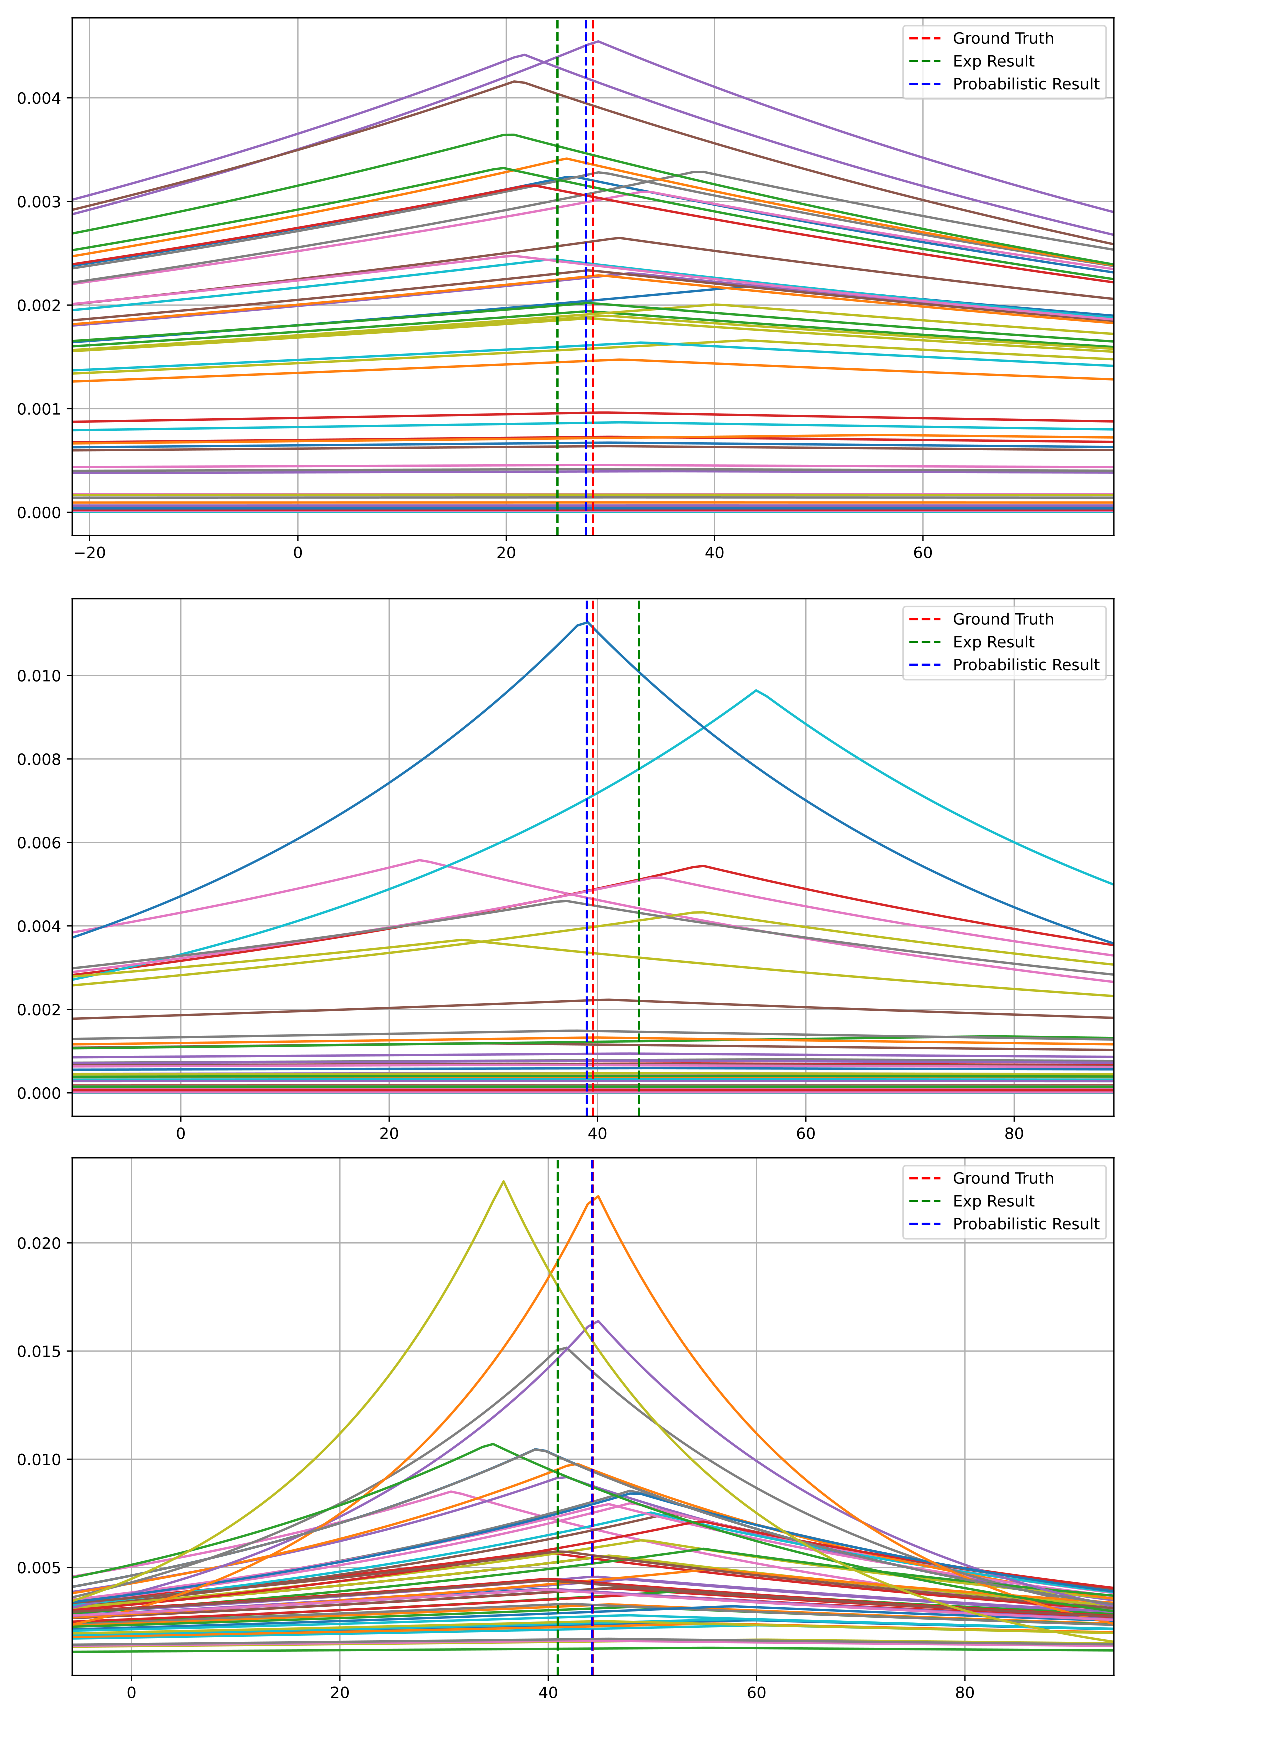
\includegraphics[width=1.0\linewidth]{ppp.eps}
		\caption{Examples of PPP modules. The red dotted line denotes the ground truth instance depth, while the green dotted line represents the predicted instance depth computed through exponential weighted summation. Our method's predicted depth is indicated by the blue dotted line.}
		\label{fig:ppp}
	\end{figure}
	
	We aim to find the optimal depth value that maximizes the likelihood of observing the predictions within a narrow range centered around it. We said we use the idea of maximum likelihood function but not direct this method, because maximum likelihood function is that we know about which distribution the real data follows, and we use the observed data to predict the distribution parameters. However, in our method, we use the predicted distribution to determine the observed position with maximum likelihood. We think our method is more like a multi-model fusion method. In Fig.~\ref{fig:ppp}, we give some examples of the application of our method.
	
	\section{Experiments}\label{sec:exp}
	\subsection{Dataset}
	\subsubsection{KITTI Dataset}
	The KITTI dataset~\cite{kitti} is widely acknowledged as a standard benchmark in the field of 3D object detection. It comprises 7,481 images paired with finely calibrated 3D bounding boxes for training, as well as 7,518 samples designated for testing. We split the training set into two subsets: a training with 3,712 samples and a validation set with 3,769 samples. This division was employed for fine-tuning and optimizing hyperparameters during model development. For the final submissions to the KITTI test server, we train the model on the whole dataset and use the weight of the last epoch.
	
	\subsubsection{Waymo Dataset}
	We perform experiments on Waymo dataset~\cite{waymo}, which is a large-scale modern dataset for self-driving. It contains 798 sequences for training and 202 sequences for validation. We sample every $3^{rd}$ frame from the training sequence to form a small training set like CaDDN. The processed training sets have approximately 50k frames.
	
	We do not perform experiments on datasets such as nuScenes~\cite{caesar2020nuscenes}, which features six cameras, as we believe that multi-view methods are more appropriate for this type of data. Our research scope does not extend to this area.
	
	
	\subsection{Implementation Details}\label{imple}
	In MSGA module, we use $1\times 1$ convolution and leaky ReLU and $1\times 1$ convolution along with a Sigmoid function to get the attention map. For enlarged RoI, we add no pixels, 5 pixels and 15 pixels, to each side of the RoI. We have test different configuration in the Sec~\ref{sec:exp}. We set $\sigma=0.1$ to refine our post processing process. The value of $\sigma$ is choosen based on the experiments. We use Adam as our optimizer, and set weight decay as 0.00001. We train our model for 200 epochs. At the first 5 epochs, we use the cosine function to transform the learning rate from 0.00001 to 0.001. The learning rate is set to 0.001 in the remaining epochs. And will decay by 0.1 at the 90 and 120 epoch. In the training phase, we remove the frame with no ground truth label for more stable and robust training. For visual depth labeling, we utilize the LRRU method~\cite{lrru} to execute depth completion, thereby generating labeled visual depth data for network training.
	
	
	\begin{figure}[!t]
		\centering
		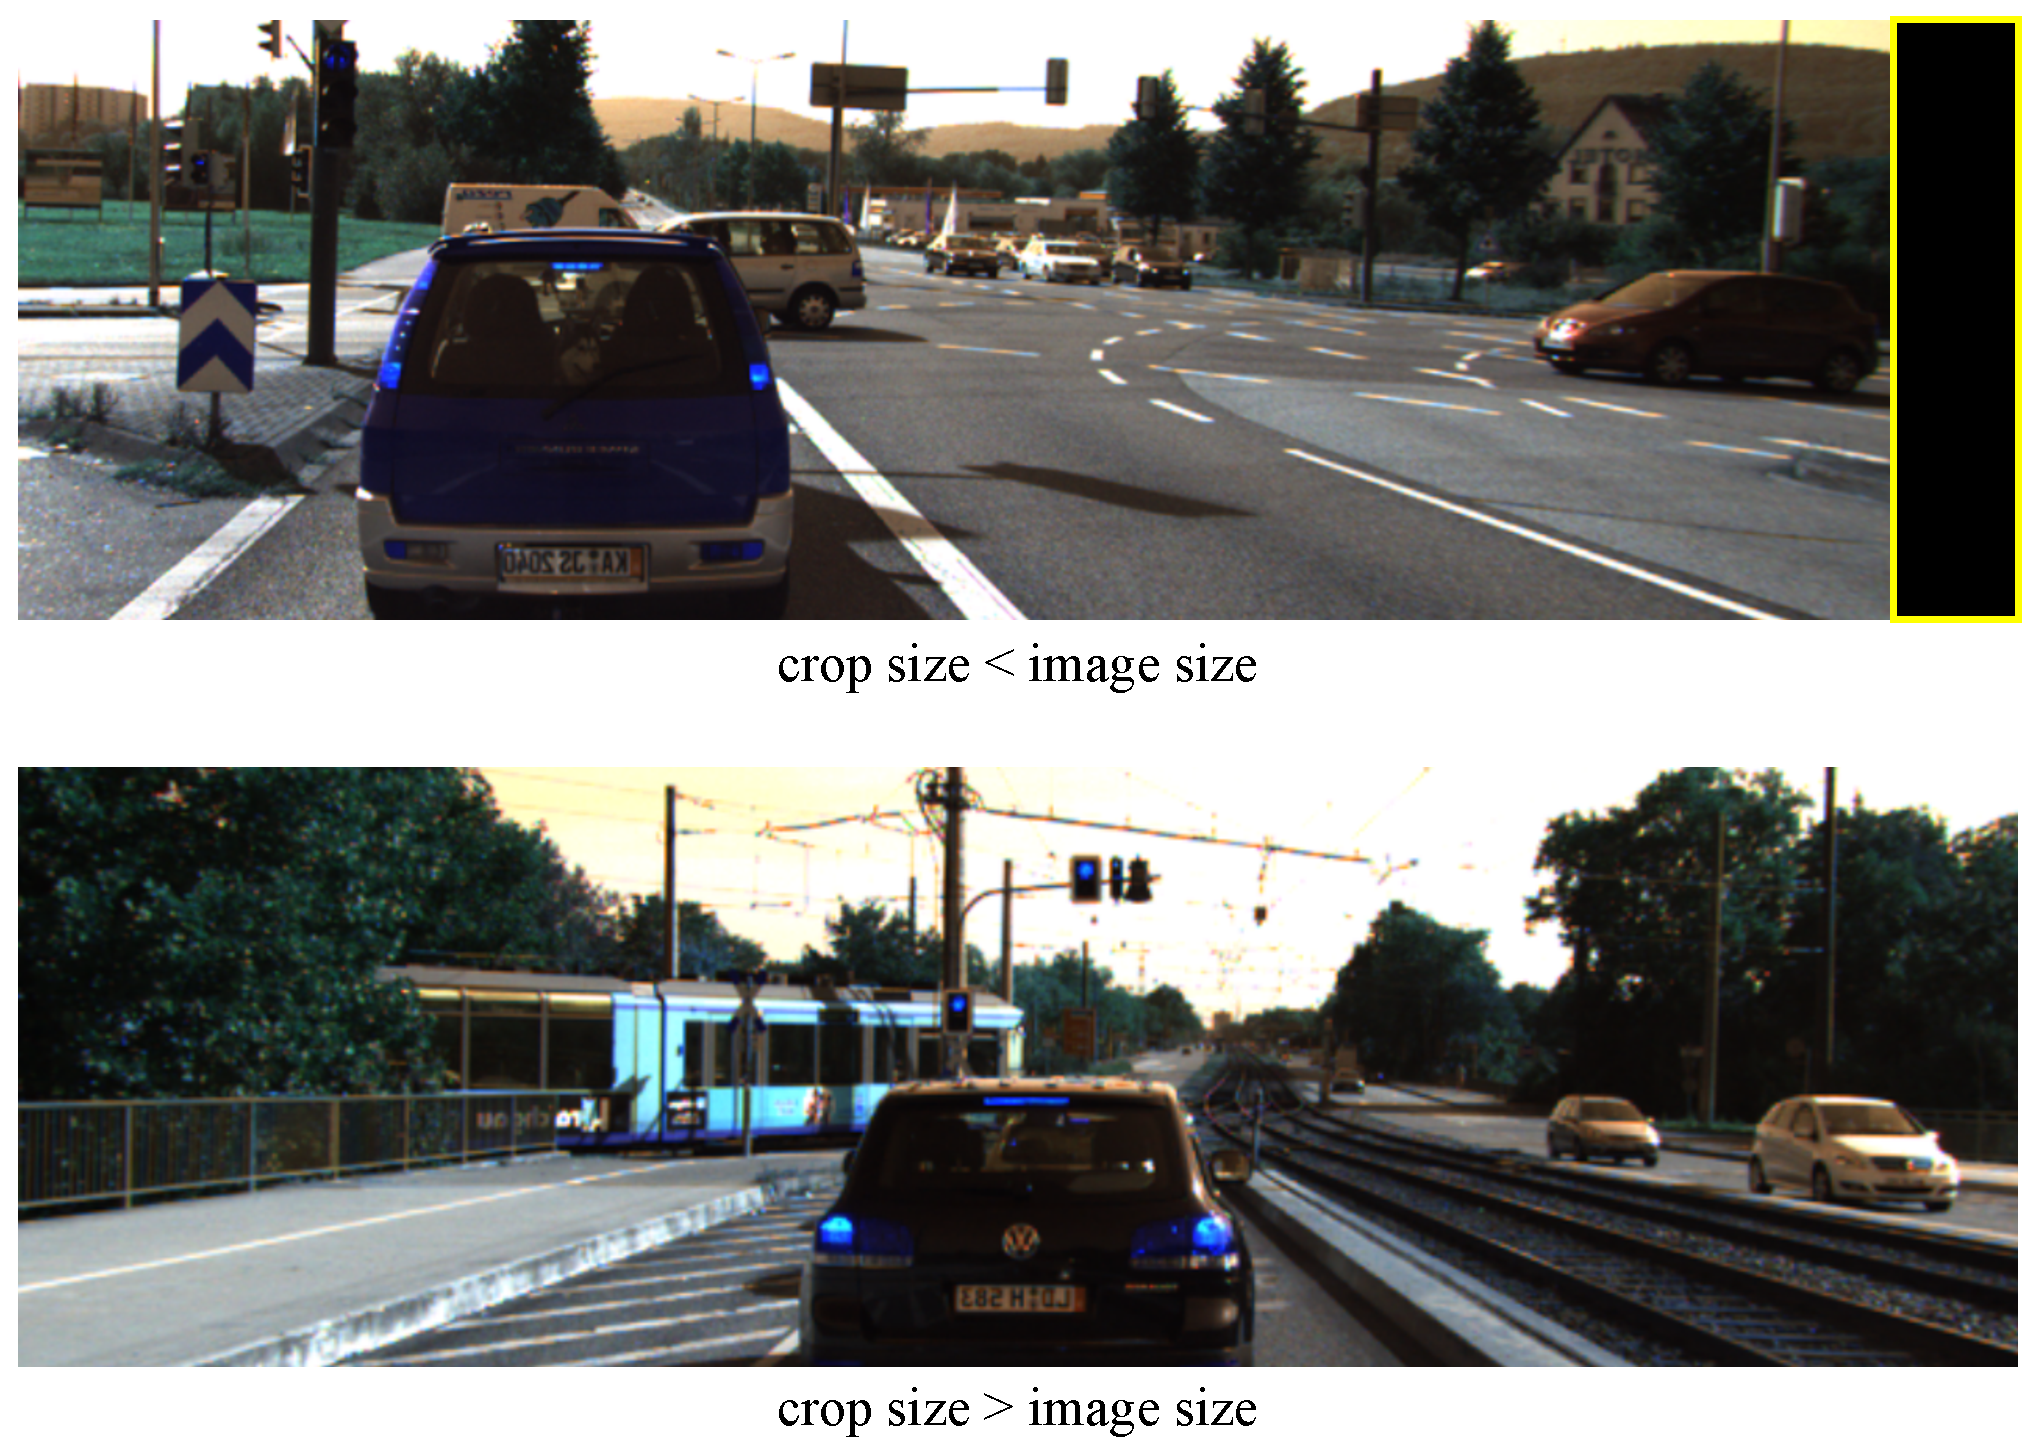
\includegraphics[width=1.0\linewidth]{affine.eps}
		\caption{Different circumstance of random cropping. When the crop size is smaller than the image size, the image is scaled to fit the crop size, resulting in black edges around the image. Conversely, if the crop size exceeds the image dimensions, the image is scaled to match the crop size, retaining only the portion within the image boundary.}
		\label{fig:affine trans}
	\end{figure}
	For data augmentation, we use random flip and random crop. After flipping and cropping, affine transformation will be applied on the cropped image to resize the image to the size of $(1280, 384)$ for batch processing. It should be noted that, after cropping and affine transformation, it may cause the processed image having black edge or remove some objects outside the picture, as depicted in Fig.~\ref{fig:affine trans}. For the first condition, for the keypoint of centerpoint that locates in the black space, we calculate their heatmap. For that outside the whole image, we do not calculate their heatmap. But in training phase, the heatmap of black edge do not participate into the loss calculation. For the second condition, if centers of all objects are outside the image, we random sample another item in the dataset.
	
	In the PPP module, optimizing depth determination is framed as an optimization problem, for which we employ the Brent algorithm~\cite{brent} to find the solution. During the training phase, we adopt the hierarchical task learning strategy introduced by GUPNet~\cite{gupnet}. This approach involves training different tasks sequentially. Initially, we focus on training the 2D object detection task, which includes generating 2D heatmaps and bounding boxes. Throughout this phase, $\lambda_{heat}$ and $\lambda_{box_{2d}}$ are both set to 1. Subsequently, the weights $\lambda_{box_{3d}}$ and $\lambda_{angle}$ are adjusted based on the convergence of 2D bounding box predictions. The weights $\lambda_{depth}$, $\lambda_{H_k}$, and $\lambda_{keypoint}$ are determined by the convergence of both 2D bounding box predictions and 3D size predictions. Further details regarding these adjustments can be found in GUPNet~\cite{gupnet}.
	\begin{table}[]
		\centering
		\caption{{Car results on KITTI Testing Dataset}}
		\label{tab:kitti_test}
		{%
			\begin{tabular}{cccccc}
				\toprule%?????
				\multirow{2}{*}{{Method}} & \multicolumn{3}{c}{{Car(IoU=0.7)}}                & \multirow{2}{*}{{3D mAP}} & \multirow{2}{*}{{Latency(ms)}} \\ \cmidrule{2-4}
				& {Easy}           & {Mod.}           & {Hard}           &                         \\ 
				\midrule%?????
				{MonoDLE~\cite{monodle}}			& {17.23}	& {12.26}	& {10.29}	& {13.29} & 40	\\
				{MonoFlex~\cite{monoflex}}			& {19.94}	& {13.89}   & {12.07}   & {15.30}	& 35 \\
				{GUPNet~\cite{gupnet}}            	& {20.11}   & {13.20}   & {11.77}   & {15.03}	& 34\\
				{MonoCon~\cite{monocon}}         	& {22.50}   & {16.46}   & {13.95}   & {17.64}	& \textbf{26} \\
				{DD3D~\cite{dd3d}}         			& {23.19}   & {16.87}   & {14.36}   & {18.14} & -	\\
				{MonoDTR~\cite{monodtr}}         	& {21.99}   & {15.39}   & {12.73}   & {16.70} & 37	\\
				{MonoPGC~\cite{monopgc}}         	& {24.68}   & {17.17}   & {14.14}   & {18.66}	& 46 \\
				{MonoDETR~\cite{monodetr}} & 25.00 & 16.47 & 13.58 & 18.35 & -
				\\
				{GUPNet++~\cite{gupnet++}}         	& {24.99}   & {16.48}   & {14.58}   & {18.68}	& -\\
				{MonoNeRD~\cite{mononerd}}         	& {22.75}   & {17.13}   & {15.63}   & {18.50} & -\\
				{FD3D~\cite{fd3d}}         	& {25.38}   & {17.12}   & {14.50}   & {19.00}	& 40 \\
				{OccupancyM3D~\cite{occupancym3d}}         	& {25.55}   & {17.02}   & {14.79}   & {19.12}	& -\\
				{MonoCD~\cite{monocd}}         	& {25.53}   & {16.59}   & {14.53}   & {18.88}	& 36\\
				{ADD~\cite{add}}         	& \textbf{25.61}   & {16.81}   & {13.79}   & {18.73}	& -\\
				{MonoUNI~\cite{monouni}}         	& {24.75}   & {16.73}   & {13.49}   & {18.32}	& -\\
				{Ours}         						& {25.43} 		& {\textbf{17.89}} 		& {\textbf{15.01}} 		& {\textbf{19.44}}   & 48	\\ 
				\bottomrule%?????
			\end{tabular}
		}
	\end{table}
	
	\begin{table*}[h]
		\centering
		\caption{{Car results on KITTI validation dataset}}
		\label{tab:kitti_valid}

			{%
				\begin{tabular}{ccccccccccccc}
					\toprule%?????
					\multirow{2}{*}{{Method}} & \multicolumn{3}{c}{{3D@IoU=0.7}} & \multicolumn{3}{c}{{BEV@IoU=0.7}}  & \multicolumn{3}{c}{{3D@IoU=0.5}} & \multicolumn{3}{c}{{BEV@IoU=0.5}}\\ \cmidrule{2-13}
					& {Easy}           & {Mod.}           & {Hard}   & {Easy}           & {Mod.}           & {Hard} & {Easy}           & {Mod.}           & {Hard} & {Easy}           & {Mod.}           & {Hard}                        \\ 
					\midrule%?????
					{MonoDLE~\cite{monodle}}			& {17.45}	& {13.66}	& {11.68}	& 24.97 & 19.33 & 17.01 & 55.41 & 43.42 & 37.81 & 60.73 & 46.87 & 41.89 	\\
					{MonoFlex~\cite{monoflex}}			& {23.64}	& {17.51}   & {14.83}  & - & - & - & - & - & - & - & - & -  	\\
					{GUPNet~\cite{gupnet}}            	& {22.76}   & {16.46}   & {13.72}  & 31.07 & 22.94 & 19.75 & 57.62 & 42.33 & 37.59 & 61.78 & 47.06 & 40.88 	\\
					{MonoCon~\cite{monocon}}         	& {26.33}   & {19.01}   & {15.98}  & - & - & - & - & - & - & - & - & -  	\\
					{MonoDTR~\cite{monodtr}}         	& {24.52}   & {18.57}   & {15.51}  & 33.33 & 25.35 & 21.68 & 64.03 & 47.32 & 42.20 & 69.04 & 52.47 & 45.90 	\\
					{MonoPGC~\cite{monopgc}}         	& {25.67}   & {18.63}   & {15.65}  & 34.06 & 24.26 & 20.78 & - & - & - & - & - & -  	\\
					{MonoDETR~\cite{monodetr}} & 28.84 & 20.61 & 16.38 & - & - & - & - & - & - & - & - & -  	\\
					
					{GUPNet++~\cite{gupnet++}}         	& \textbf{29.03}   & {20.45}   & {17.89}  & 38.82 & 27.95 & 24.96 & 66.66 & 49.65 & 45.23 & 71.55 & 54.00 & 49.34 	\\
					{OccupancyM3D~\cite{occupancym3d}}         	& {26.87}   & {19.96}   & {17.15}  & 35.72 & 26.60 & 23.68 & - & - & - & - & - & - 	\\
					{MonoCD~\cite{monocd}}         	& {24.22}   & {18.27}   & {15.42}  & - & - & - & - & - & - & - & - & - 	\\
					{FD3D~\cite{fd3d}}         	& {28.22}   & {20.23}   & {17.04}  & 36.98 & 26.77 & 23.16 & - & - & - & - & - & - 	\\
					{MonoUNI~\cite{monouni}}         	& {24.51}   & {17.18}   & {14.01}  & - & - & - & - & - & - & - & - & - 	\\
					{Ours}         						& {28.93} 		& \textbf{21.07} 		& \textbf{18.13} & \textbf{39.34} 	& \textbf{28.58} & \textbf{25.89} & \textbf{67.44} & \textbf{51.37} & \textbf{46.88} & \textbf{72.34} & \textbf{55.13} & \textbf{50.23}	   	\\ 
					\bottomrule%?????
				\end{tabular}
			}

	\end{table*}
	
	
	% Please add the following required packages to your document preamble:
	% \usepackage{multirow}
	% \usepackage{graphicx}
	\begin{table*}[h]
		\centering
		\setlength{\tabcolsep}{1mm}
		\caption{Results of Waymo Validation Dataset}
		\label{tab:waymo_valid}
		
		{%
			\begin{tabular}{ccccc}
				\toprule%?????
				\multirow{2}{*}{Methods} & \multicolumn{4}{c}{3D mAP/mAPH}       \\ \cmidrule{2-5}
				& Overall & 0-30m & 30-50m & 50m-$\inf$ \\
				\midrule%?????
				
				\multicolumn{5}{c}{Under Level 1(IoU=0.5)}                       \\
				\midrule%?????
				
				PatchNet~\cite{patchnet}              & {2.92/2.74}  	 & {10.01/9.75} 	 & {1.09/0.96} 		 & {0.23/0.18}	\\
				CaDDN~\cite{caddn}                    & {17.54/17.31}    & \textbf{45.00/44.46}     & {9.24/9.11}       & {0.64/0.62}	\\
				PCT~\cite{pct}                     	  & {4.20/4.15}      & {14.70/14.54}     & {1.78/1.75}       & {0.39/0.39}  \\
				MonoJSG~\cite{monojsg}                & {5.65/5.47}      & {20.86/20.26}     & {3.91/3.79}       & {0.97/0.92}  \\
				SSD-MonoDETR~\cite{ssd-monodetr}      & {11.83/-}    	 & {27.69/-}         & {5.33/-}          & {0.85/-}     \\
				MonoUNI~\cite{monouni}                 & {10.98/10.73}    & {26.63/26.30}     & {4.04/3.98}     & {0.57/0.55}  \\
				DID-M3D~\cite{didm3d}                 & {20.66/20.47}    & {40.92/40.60}     & {15.63/15.48}     & {5.35/5.24}  \\
				Ours					 			  &	\textbf{22.69/22.33}	 & {43.27/42.89}	 &	\textbf{16.94/16.72} &	\textbf{6.38/6.12}	 			\\
				\midrule%?????
				\multicolumn{5}{c}{Under Level 2(IoU=0.5)}                       \\
				\midrule%?????
				PatchNet~\cite{patchnet}              & {2.42/2.28}      & {10.01/9.73}      & {1.07/0.94}       & {0.22/0.16}  \\
				CaDDN~\cite{caddn}                    & {16.51/16.28}    & \textbf{44.87/44.33}     & {8.99/8.86}       & {0.58/0.55}	\\
				PCT~\cite{pct}                        & {4.03/3.99}      & {14.67/14.51}     & {1.74/1.71}       & {0.36/0.35}  \\
				MonoJSG~\cite{monojsg}                & {5.34/5.17}      & {20.79/20.19}     & {3.79/3.67}       & {0.85/0.82}  \\
				SSD-MonoDETR~\cite{ssd-monodetr}      & {11.34/-}    	 & {27.62/-}     	 & {5.21/-}          & {0.76/-}     \\
				MonoUNI~\cite{monouni}                 & {10.38/10.24}    & {26.57/26.24}     & {3.95/3.89}     & {0.53/0.51}  \\
				DID-M3D~\cite{didm3d}                 & {19.37/19.19}    & {40.77/40.46}     & {15.18/15.04}     & {4.69/4.59}	\\
				Ours & \textbf{21.47/21.33} & {42.39/42.14} & \textbf{16.53/16.37} &\textbf{5.12/5.01}			 								 									\\
				\bottomrule%?????
			\end{tabular}%
		}
	\end{table*}
	\subsection{Experiment Results}
	\subsubsection{KITTI Test Dataset}
	We perform experiments on the KITTI test dataset and present the comparison between our method and state-of-the-art approaches in Table~\ref{tab:kitti_test}, with the best results highlighted in bold. The results demonstrate that our method surpasses others, with the exception of the Easy category, where ADD~\cite{add} shows superior results. We attribute this to the fact that ADD employs knowledge distillation, which is particularly effective in learning from the teacher network for the more straightforward parts of the task. Additionally, our method achieves real-time performance (less than 50ms) without requiring any acceleration strategies, which is acceptable for practical applications.
	
	\subsubsection{KITTI Validation Dataset}
	
	Experiments were conducted on the KITTI validation dataset, and the results are presented in Table~\ref{tab:kitti_valid}, with superior outcomes highlighted in bold. Our method demonstrates superior performance across most metrics, except for the Easy subset with 0.7 IoU threshold. However, on the test dataset, our model outperforms GUPNet++ across all metrics. This suggests that GUPNet++ may suffer from slight overfitting, resulting in a smaller performance gap between our method and theirs on the validation dataset.
	
	\subsubsection{Waymo Validation Dataset}
	
	Experiments are conducted on the Waymo validation dataset, and the comparison between our method and other approaches is presented in Table~\ref{tab:waymo_valid}, with the best results highlighted in bold. Since many other methods only conduct experiments on a subset of the Waymo Dataset, we adopt the same strategy for fair comparison. The results shows that our methods outperform other methods except CaDDN in 0-30m. We think that this is because CaDDN use the depth classification for depth estimation, and this type of method will may more attention to the near objects, and our methods treat the objects in different distances more balanced.
	
	\begin{table}[]
		\centering
		\setlength{\tabcolsep}{1mm}
		\caption{Effects of different components}
		\label{tab:diff_com}
		{%
			\begin{tabular}{cccccccc}
				
				\hline
				\multirow{2}{*}{{No.}}  & \multirow{2}{*}{MS}       & \multirow{2}{*}{GA}      & \multirow{2}{*}{PPP}       & \multicolumn{3}{c}{{Car (IoU=0.7)}} & \multirow{2}{*}{3D mAP} \\ \cmidrule{5-7}
				& &                           &                           & Easy  & Mod.  & Hard  &       \\ \hline
				{(a)}&   			&              &              	& 26.46 & 18.43 & 15.32 &  20.07	\\
				{(b)}& \checkmark   &              &              	& 27.56 & 19.32 & 15.98 &  20.95	\\
				{(c)}& 				& 	\checkmark &				& 27.23 & 19.01 & 16.47 &  20.90 	\\
				{(d)}& 				&              & \checkmark 	& 27.34 & 19.45 & 16.35 &  21.05	\\
				{(e)}& {\checkmark} &{\checkmark}  & 			 	& 28.12 & 20.31 & 17.12 &  21.85 	\\
				{(f)}&           	&{\checkmark}  & {\checkmark} 	& 28.33 & 20.45 & 17.56 &  22.11 	\\
				{(g)}&{\checkmark}  &              & {\checkmark} 	& 28.42 & 20.44 & 17.43 &  22.10	\\
				{(h)}&\checkmark    & \checkmark   & \checkmark     & \textbf{28.93} & \textbf{21.07} 		&\textbf{18.13} & \textbf{22.71}	\\ \hline
			\end{tabular}%
		}
	\end{table}
	
	\begin{table}[]
		\centering
		\setlength{\tabcolsep}{1mm}
		\caption{Effects of Multi-Scale Methods}
		\label{tab:multi scale}
		{%
			\begin{tabular}{cccccccc}
				\hline
				\multirow{2}{*}{{FT}}  & \multirow{2}{*}{CD} & \multirow{2}{*}{Scale} & \multicolumn{3}{c}{{Car (IoU=0.7)}} & \multirow{2}{*}{3D mAP} \\ \cmidrule{4-6} & & & Easy  & Mod.  & Hard  &       \\ \hline
				5		&5		&-						& 28.67 & 20.88 & \textbf{18.23} & 22.59 	\\
				5		&10		&-						& {28.93} & \textbf{21.07} 		&{18.13} & \textbf{22.71}	\\
				5		&15		&-						& 28.88 & 20.78 & 17.69 & 22.45 	\\
				10		&5		&-						& 28.91 & 20.83 & 17.54 & 22.43 	\\
				10		&10		&-						& \textbf{29.01} & 20.75 & 17.49 & 22.42 	\\
				10		&15		&-						& 28.74 & 20.69 & 16.58 & 20.00 	\\
				15		&5		&-						& 28.63 & 20.83 & 16.79 & 22.08 	\\
				15		&10		&-						& 28.66 & 20.66 & 16.54 & 21.95 	\\
				15		&15		&-						& 28.74 & 20.88 & 16.32 & 21.98 	\\ 
				-		&-		&(1.0, 1.05, 1.1)		& 25.42 & 17.56 & 14.49 & 19.16 	\\ 
				-		&-		&(1.1, 1.2, 1.3)		& 24.95 & 16.69 & 13.78 & 18.47 	\\ \hline
			\end{tabular}%
		}
	\end{table}
	
	\begin{table}[]
		\centering
		\caption{Effects of Different Attention Mechanism}
		\label{tab:attention mechanism}
		{%
			\begin{tabular}{ccccc}
				\hline
				\multirow{2}{*}{{Method}} & \multicolumn{3}{c}{{Car (IoU=0.7)}} & \multirow{2}{*}{3D mAP} \\ \cmidrule{2-4}
				& Easy  & Mod.  & Hard  &       \\ \hline
				Self Attention 		& {28.51} & {20.12} 		&{16.34} & {21.66} 	\\
				Learn Query Attention 	& 28.12 & 20.01 & 16.12 & 21.42 	\\
				Ours 			&  \textbf{28.93} & \textbf{21.07} 		&\textbf{18.13} & \textbf{22.71} 	 	\\\hline
			
			\end{tabular}%
		}
	\end{table}
	
	\begin{table}[]
		\centering
		\caption{Effects of Grid Attention Activation Function}
		\label{tab:grid attention activate function}
		{%
			\begin{tabular}{ccccc}
				\hline
				\multirow{2}{*}{{Method}} & \multicolumn{3}{c}{{Car (IoU=0.7)}} & \multirow{2}{*}{3D mAP} \\ \cmidrule{2-4}
				& Easy  & Mod.  & Hard  &       \\ \hline
				Sigmoid 		& {28.93} & \textbf{21.07} 		&\textbf{18.13} & \textbf{22.71} 	\\
				Hard Sigmoid 	& 28.74 & 21.05 & 17.74 & 22.51 	\\
				Tanh 			& \textbf{29.03} & 20.94 & 17.99 & {22.65}  	\\
				Softmax			& 27.93 & 20.66 & 17.32 & {21.97}  	\\ \hline
			\end{tabular}%
		}
	\end{table}
	
	\begin{table}[]
		\centering
		\caption{Effects of Probabilistic Post Processing}
		\label{tab:ppp module}
		{%
			\begin{tabular}{ccccc}
				\hline
				\multirow{2}{*}{{Method}} & \multicolumn{3}{c}{{Car (IoU=0.7)}} & \multirow{2}{*}{3D mAP} \\ \cmidrule{2-4}
				& Easy  & Mod.  & Hard  &       \\ \hline
				$\delta$=0.05 		& {27.95} & {20.13} 		&{16.54} & {21.54}  	\\
				$\delta$=0.1 		& \textbf{28.93} & \textbf{21.07} 		&\textbf{18.13} & \textbf{22.71}  	\\
				$\delta$=0.2 		& 28.66 & 20.73 & 17.63 & 22.34 	\\
				$\delta$=0.3  		& 28.65 & 20.76 & 17.79 & 22.40  	\\
				$\delta$=0.4 		& 28.03 & 20.24 & 17.02 & 21.76  	\\ \hline
			\end{tabular}%
		}
	\end{table}
	
	\subsection{Ablation Studies}
	\subsubsection{Influence of different components}
	We evaluated the MSGA and PPP modules as presented in Table~\ref{tab:diff_com}. Our baseline model, without these modules, serves as a reference point. Results from experiments (b), (c) and (d) demonstrate that incorporating either module individually enhances performance. Moreover, for combinations involving both modules, such as (e), (f) and (g), those with PPP exhibit superior performance compared to those without. This suggests that probabilistic information plays a crucial role in network learning, particularly for models with probabilistic assumptions. Experiment (h) indicates that the model incorporating all modules achieves the highest performance, highlighting the effectiveness of our proposed modules in directing attention to RoI grids and leveraging probabilistic cues more effectively.
	
	
	\subsubsection{Influence of Multi-Scale Methods}
	We tested the impact of enlarging the RoI on performance. Initially, we uniformly increased both the width and height by the same number of pixels, and also explored proportionally enlarging the RoI. Our findings revealed a significant performance drop when enlarging the bounding box by factors of 1.0, 1.05, and 1.1. Further proportional increases exacerbated this decline due to scale variance in the image plane. Conversely, when adopting a strategy of enlarging the RoI by a fixed number of pixels, we devised a scheme to generate additional pixels in a multi-scale fashion, forming an arithmetic series based on the First Term (FT) and the Common Difference (CD). The experiment is depicted in Table~\ref{tab:multi scale}. Increasing the FT and CD led to deteriorating performance in hard partitions. This is likely because objects in hard partitions typically have small 2D bounding boxes, causing background pixels to dominate the learning process when more pixels are added. Conversely, changes in FT and CD had less impact on easy and moderate partitions, consistent with our assumption that objects in these partitions have larger 2D bounding boxes, making minor pixel adjustments less influential. Proportionally enlarging the bounding box resulted in notably worse performance compared to our methods, attributed to scale variance in the image plane. Even in hard partitions where bounding boxes are small, performance was inferior to simply adding fixed pixels. This discrepancy may stem from the network's confusion regarding background and foreground pixels due to varying bounding box sizes and the corresponding distribution of background and foreground pixels within the enlarged bounding box. The prevalence of large objects outweighs that of small objects, indicating an imbalance in object sizes. Proportionally enlarging RoIs exacerbates this issue, resulting in a significant increase in background pixels. Consequently, the network might inadvertently learn the relative proportion of background to foreground pixels. This can lead to confusion during the processing of small objects, hindering the model's learning process.
	
	\subsubsection{Influence of Different Attention Mechanism}
	We explored alternative attention mechanisms by replacing the attention map in the MSGA module with self-attention and learned query attention, while retaining the multi-scale strategy. Self-attention refers to the basic mechanism used in Transformer~\cite{transformer}, while learned query attention, as used in DETR~\cite{detr}, replaces the RoI feature with learned parameters as the query. These learned parameters are then used in place of the RoI feature in the attention mechanism.
	
	Our experiments show that the simplest sigmoid attention performs better than the others. We attribute this to the relatively uniform relationships between RoI grids. Since we are predicting the depth of each grid, no single grid holds an obvious clue, and the information might be distributed across many grids. The softmax function in the other two attention mechanisms tends to distribute attention uniformly, which aligns with our experimental samples. This suggests that complex global dependencies are unnecessary. As shown in Fig~\ref{fig:multi-scale-grid-attention}, the simplest sigmoid attention provides reasonable attention to the grids, highlighting the importance of foreground over background.
	
	\subsubsection{Influence of Grid Attention Activation Function}
	To scale the output of the attention map to the range $[0, 1]$, we evaluate several activation functions for comparison, as detailed in Table~\ref{tab:grid attention activate function}. Sigmoid, Hard Sigmoid~\cite{hard-sigmoid}, and Softmax are directly applied to the attention map. However, since the Tanh function maps values to the range $[-1, 1]$, we employ the transformation outlined in Eq.~\eqref{eq:tanh} to map these values to $[0, 1]$.
	\begin{equation}
		\begin{aligned}
			att = (1+tanh(x))/2,
			\label{eq:tanh}
		\end{aligned}
	\end{equation}
	
	where $att$ is the attention map, $x$ is the output of the network.
	
	The experimental results are presented in Table~\ref{tab:grid attention activate function}. Sigmoid, hard sigmoid, and tanh functions exhibit comparable performance, while the softmax function performs notably worse. This discrepancy can be attributed to the softmax function's tendency to assign high attention to one grid and low attention to others. However, since the RoI is not determined solely by one grid, this approach proves less effective.
	
	\subsubsection{Influence of Probabilistic Posting Processing}
	We selected the hyper-parameters $\delta$ in the Probabilistic Post-Processing (PPP) module to optimize its performance. If $\delta$ is too small, the model tends to focus solely on predictions with the lowest uncertainty. Conversely, if $\delta$ is too large, the differences between positions become less discernible. The experimental findings are detailed in Table~\ref{tab:ppp module}. Setting $\delta$ to values such as 0.05 or 0.4 leads to a drop in performance. Consequently, we determined that $\delta=0.1$ yields the best results based on our experiments.
	
	\section{Future Work}\label{future work}
	While our proposed method has demonstrated significant improvements in the accuracy and robustness of monocular 3D object detection, there are several limitations that suggest promising directions for future research:
	
	\textbf{Depth Completion Network Refinement}: Our approach relies on an independent depth completion network to generate ground truth visual depth. The accuracy of this network is crucial, as errors in depth estimation can propagate through our system. Future work could focus on enhancing the depth completion network, potentially through the incorporation of more sophisticated neural architectures or additional training strategies.
		
	\textbf{Denoising of Training Data}: As our method can be sensitive to noise in the depth estimation network, research into denoising techniques or the use of synthetic data to augment training sets could improve model robustness.
	
	\section{Conclusion}\label{conclusion}
	In this paper, we delve into the challenges of RoI-based monocular 3D object detection. We identify two main issues: errors in 2D bounding box prediction and overlooked variations in RoI grid weights, hindering effective network learning. To address these issues, we introduce the MSGA module, which allocates grid attention intelligently and integrates multi-scale features to mitigate prediction errors. Additionally, acknowledging the probabilistic assumptions prevalent in existing methods, we propose the PPP module to better leverage probabilistic cues. Both modules significantly enhance baseline performance.
	
	\section{Acknowledgements}
	This study is supported in part by the National Natural Science Foundation of China (62272194, 62172186), and in part by the Science and Technology Development Plan Project of Jilin Province (20220101101JC). 
	
	%\bibliographystyle{IEEEtran}
	%\bibliography{references.bib}
	\begin{thebibliography}{1}
		\bibliographystyle{IEEEtran}	
		\bibitem{geometry3d}
		A. Mousavian, D. Anguelov, J. Flynn and J. Kosecka, “3d bounding box estimation using deep learning and geometry,” in \textit{Proc. IEEE/CVF Conf. Comput. Vis. Pattern Recognit.}, Honolulu, HI, USA, 2017, pp. 7074-7082.
		
		\bibitem{roi10d}
		F. Manhardt, W. Kehl and A. Gaidon, “Roi-10d: Monocular lifting of 2d detection to 6d pose and metric shape,” in \textit{Proc. IEEE/CVF Conf. Comput. Vis. Pattern Recognit.}, Long Beach, CA, USA. 2019, pp. 2069-2078.
		
		\bibitem{monopair}
		Y. Chen, L. Tai, K. Sun and M. Li, “Monopair: Monocular 3d object detection using pairwise spatial relationships,” in \textit{Proc. IEEE/CVF Conf. Comput. Vis. Pattern Recognit.}, Seattle, WA, USA, 2020, pp. 12093-12102.
		
		\bibitem{smoke}
		Z. Liu, Z. Wu and R. Tóth, “Smoke: Single-stage monocular 3d object detection via keypoint estimation,” in \textit{Proc. IEEE/CVF Conf. Comput. Vis. Pattern Recognit.}, Seattle, WA, USA, 2020, pp. 996-997.
		
		\bibitem{polygon}
		Y. Cai, B. Li, Z. Jiao, H. Li, X. Zeng and X. Wang, “Monocular 3d object detection with decoupled structured polygon estimation and height-guided depth estimation,” in \textit{Proc. AAAI Conf. Artif. Intell.}, New York, USA, 2020, pp. 10478-10485.
		
		\bibitem{monoflex}
		Y. Zhang, J. Lu and J. Zhou, “Objects are different: Flexible monocular 3d object detection,” in \textit{Proc. IEEE/CVF Conf. Comput. Vis. Pattern Recognit.}, Nashville, TN, USA, 2021, pp. 3289-3298.
		
		\bibitem{caddn}
		C. Reading, A. Harakeh, J. Chae and SL. Waslander, “Categorical depth distribution network for monocular 3d object detection,” in \textit{Proc. IEEE/CVF Conf. Comput. Vis. Pattern Recognit.}, Nashville, TN, USA, 2021, pp. 8555-8564.
		
		\bibitem{gupnet}
		Y. Lu et al., “Geometry uncertainty projection network for monocular 3d object detection,” in \textit{Proc. IEEE/CVF Int. Conf. Comput. Vis.}, Montreal, Canada. 2021, pp. 3111-3121.
		
		\bibitem{dd3d}
		D. Park, R. Ambrus, V. Guizilini, J. Li and A. Gaidon, “Is pseudo-lidar needed for monocular 3d object detection?,” in \textit{Proc. IEEE/CVF Int. Conf. Comput. Vis.}, Montreal, Canada. 2021, pp. 3142-3152.
		
		\bibitem{monodde}
		Z. Li, Z. Qu, Y. Zhou, J. Liu, H. Wang and L. Jiang, “Diversity matters: Fully exploiting depth clues for reliable monocular 3d object detection,” in \textit{Proc. IEEE/CVF Conf. Comput. Vis. Pattern Recognit.}, New Orleans, LA, USA, 2022, pp. 2791-2800.
		
		\bibitem{didm3d}
		L. Peng, X. Wu, Z. Yang, H. Liu and D. Cai, “Did-m3d: Decoupling instance depth for monocular 3d object detection,” in \textit{Eur. Conf. Comput. Vis.}, Tel-Aviv, Israel, 2022, pp. 71–88.
		
		\bibitem{imvoxelnet}
		D. Rukhovich, A. Vorontsova and A. Konushin, “Imvoxelnet: Image to voxels projection for monocular and multi-view general-purpose 3d object detection,” in \textit{Proc. IEEE/CVF Winter Conf. Appl. Comput. Vis.}, Waikoloa, HI, USA. 2022, pp. 2397-2406.
		
		\bibitem{pgd}
		T. Wang, ZHU. Xinge, J. Pang and D. Lin, “Probabilistic and geometric depth: Detecting objects in perspective,” in \textit{Conf. on Robot. Learn.}, London, UK, 2022, pp. 1475-1485.
		
		\bibitem{monodtr}
		KC. Huang, TH. Wu, HT. Su and WH. Hsu, “Monodtr: Monocular 3d object detection with depth-aware transformer,” in \textit{Proc. IEEE/CVF Conf. Comput. Vis. Pattern Recognit.}, New Orleans, LA, USA, 2022,  pp. 4012-4021.
		
		
		\bibitem{monocon}
		X. Liu, N. Xue and T. Wu, “Learning auxiliary monocular contexts helps monocular 3d object detection,” in \textit{Proc. AAAI Conf. Artif. Intell.}, Vol. 36, No. 2, Virtual, 2022, pp. 1810-1818.
		
		\bibitem{cie}
		Q. Ye, L. Jiang, W. Zhen and Y. Du, “Consistency of implicit and explicit features matters for monocular 3d object detection,” 2022, \textit{arXiv:2207.07933}.
		
		\bibitem{monoxiver}
		X. Liu, C. Zheng, KB. Cheng, N. Xue, GJ. Qi and T. Wu, “Monocular 3d object detection with bounding box denoising in 3d by perceiver,” in \textit{Proc. IEEE/CVF Int. Conf. Comput. Vis.}, Paris, France. 2023, pp. 6436-6446.
		
		\bibitem{neurocs}
		Z. Min, B. Zhuang, S. Schulter, B. Liu, E. Dunn and M. Chandraker, “Neurocs: Neural nocs supervision for monocular 3d object localization,” in \textit{Proc. IEEE/CVF Conf. Comput. Vis. Pattern Recognit.}, Vancouver, Canada. 2023, pp. 21404-21414. 
		
		\bibitem{mononerd}
		J. Xu et al., “Mononerd: Nerf-like representations for monocular 3d object detection,” in \textit{Proc. IEEE/CVF Int. Conf. Comput. Vis.}, Paris, France. 2023, pp. 6814-6824. 
		
		\bibitem{monopgc}
		Z. Wu, Y. Gan, L. Wang, G. Chen and J. Pu, “Monopgc: Monocular 3d object detection with pixel geometry contexts,” in \textit{Int. Conf. Robot. Automat.}, London, UK. 2023, pp. 4842-4849. 
		
		\bibitem{gupnet++}
		Y.Lu et al., “GUPNet++: Geometry Uncertainty Propagation Network for Monocular 3D Object Detection,” in \textit{Int. Conf. Robot. Automat.}, 2023, \textit{arXiv:2310.15624}.
		
		\bibitem{ssd-monodetr}
		X. He et al., “Ssd-monodetr: Supervised scale-aware deformable transformer for monocular 3d object detection,” in \textit{IEEE Trans. Intell. Veh.}, vol. 9, no. 1, pp. 555-567, Ian. 2024, doi: 10.1109/TIV.2023.3311949.
		
		\bibitem{mask-rcnn}
		K. He, G. Gkioxari, P. Dollar and R. Girshick, “Mask r-cnn,” in \textit{Proc. IEEE/CVF Int. Conf. Comput. Vis.}, Venice, Italy. 2017, pp. 2961-2969.
		
		\bibitem{patchnet}
		X. Ma, S. Liu, Z. Xia, H. Zhang and X. Zeng, “Rethinking pseudo-lidar representation,” in \textit{Eur. Conf. Comput. Vis.}, Virtual, 2020, pp. 311–327.
		
		\bibitem{pct}
		L. Wang et al., “Progressive coordinate transforms for monocular 3d object detection,” in \textit{Adv. Neural Inf. Process. Syst.}, Vol. 34, pp. 13364--13377, 2021.
		
		\bibitem{monojsg}
		Q. Lian, P. Li and X. Chen, “Monojsg: Joint semantic and geometric cost volume for monocular 3d object detection,” in \textit{Proc. IEEE/CVF Conf. Comput. Vis. Pattern Recognit.}, New Orleans, LA, USA, 2022, pp. 1070-1079.
		
		\bibitem{tits monopixel}
		Y. Kim, S. Kim, S. Sim, J. W. Choi and D. Kum, “Boosting Monocular 3D Object Detection With Object-Centric Auxiliary Depth Supervision,” in \textit{IEEE Trans. Intell. Transp. Syst.}, vol. 24, no. 2, pp. 1801-1813, Feb. 2023, doi: 10.1109/TITS.2022.3224082.
		
		\bibitem{fast-rcnn}
		R. Girshick, “Fast r-cnn,” in \textit{Proc. IEEE/CVF Int. Conf. Comput. Vis.}, Santiago, Chile. 2015, pp. 1440-1448.
		
		\bibitem{roi-warp}
		J. Dai, K. He and J. Sun, “Instance-aware semantic segmentation via multi-task network cascades,” in \textit{Proc. IEEE/CVF Conf. Comput. Vis. Pattern Recognit.}, Las Vegas, NV, USA, 2016, pp. 3150-3158.
		
		\bibitem{tits survey}
		E. Arnold, O. Y. Al-Jarrah, M. Dianati, S. Fallah, D. Oxtoby and A. Mouzakitis, “A Survey on 3D Object Detection Methods for Autonomous Driving Applications,” in \textit{IEEE Trans. Intell. Transp. Syst.}, vol. 20, no. 10, pp. 3782-3795, Oct. 2019, doi: 10.1109/TITS.2019.2892405.
		
		\bibitem{kitti}
		A. Geiger, P. Lenz, and R. Urtasun, “Are we ready for autonomous driving? the kitti vision benchmark suite,” in \textit{Proc. IEEE/CVF Conf. Comput. Vis. Pattern Recognit.}, Providence, RI, 2012, pp. 3354–3361.
		
		\bibitem{m3d-rpn}
		G. Brazil and X. Liu, “M3d-rpn: Monocular 3d region proposal network for object detection,” in \textit{Proc. IEEE/CVF Int. Conf. Comput. Vis.}, Seoul, Korea. 2019, pp. 9287-9296.
		
		\bibitem{d4lcn}
		M. Ding, et.al., “Learning depth-guided convolutions for monocular 3d object detection,” in \textit{Proc. IEEE/CVF Conf. Comput. Vis. Pattern Recognit.}, Seattle, WA, USA, 2020, pp. 1000-1001.
		
		\bibitem{oft}
		T. Roddick, A. Kendall and R. Cipolla, “Orthographic feature transform for monocular 3d object detection,” 2018, \textit{arXiv:1811.08188}.
		
		\bibitem{color-embeded}
		X. Ma, Z. Wang, H. Li, P. Zhang, W. Ouyang and X, Fan, “Accurate monocular 3d object detection via color-embedded 3d reconstruction for autonomous driving,” in \textit{Proc. IEEE/CVF Int. Conf. Comput. Vis.}, Seoul, Korea. 2019, pp. 6851-6860.
		
		\bibitem{tits aux}
		JH. Chen, JL. Shieh, MA. Haq, SJ. Ruan, “Monocular 3D Object Detection Utilizing Auxiliary Learning With Deformable Convolution,” in \textit{IEEE Trans. Intell. Transp. Syst.}, vol. 25, no. 3, pp. 2424-2436, March 2024, doi: 10.1109/TITS.2023.3319556.
		
		\bibitem{mono-plidar}
		X. Weng, K. Kitani, “Monocular 3d object detection with pseudo-lidar point cloud,” in \textit{Proc. IEEE/CVF Int. Conf. Comput. Vis. Workshop}, Seoul, Korea. 2019.
		
		\bibitem{rtm3d}
		P. Li, H. Zhao, P. Liu and F. Cao, “Rtm3d: Real-time monocular 3d detection from object keypoints for autonomous driving,” in \textit{Eur. Conf. Comput. Vis.}, Virtual, 2020, pp. 644-660.
		
		\bibitem{tits shape aware}
		W. Chen, J. Zhao, W. -L. Zhao and S. -Y. Wu, “Shape-Aware Monocular 3D Object Detection,” in \textit{IEEE Trans. Intell. Transp. Syst.}, vol. 24, no. 6, pp. 6416-6424, June 2023, doi: 10.1109/TITS.2023.3249909.
		
		

		
		\bibitem{tits cman}
		Y. Cao, H. Zhang, Y. Li, C. Ren and C. Lang, “CMAN: Leaning Global Structure Correlation for Monocular 3D Object Detection,” in \textit{IEEE Trans. Intell. Transp. Syst.}, vol. 23, no. 12, pp. 24727-24737, Dec. 2022, doi: 10.1109/TITS.2022.3205446.
		

		
		\bibitem{nerf}
		B. Mildenhall, PP. Srinivasan, M. Tancik, JT. Barron, R. Ramamoorthi and R. Ng, “Nerf: Representing scenes as neural radiance fields for view synthesis,” in \textit{Commun. ACM}, vol. 65, no. 1, pp. 99–106, 2021.
		
		\bibitem{monodle}
		X. Ma et.al., “Delving into localization errors for monocular 3d object detection,” in \textit{Proc. IEEE/CVF Conf. Comput. Vis. Pattern Recognit.}, Nashville, TN, USA, 2021, pp. 4721-4730.
		
		\bibitem{tits plane cons}
		H. Yao et al., "Occlusion-Aware Plane-Constraints for Monocular 3D Object Detection," in \textit{IEEE Trans. Intell. Transp. Syst.}, vol. 25, no. 5, pp. 4593-4605, May 2024, doi: 10.1109/TITS.2023.3323036.
		
		\bibitem{m3dssd}
		S. Luo, H. Dai, L. Shao and Y. Ding, “M3dssd: Monocular 3d single stage object detector,” in \textit{Proc. IEEE/CVF Conf. Comput. Vis. Pattern Recognit.}, Nashville, TN, USA, 2021, pp. 6145-6154.
		
		\bibitem{tits depth estimation}
		Y. Ji and J. Xu, “Depth Estimation From Surface-Ground Correspondence for Monocular 3D Object Detection,” in \textit{IEEE Trans. Intell. Transp. Syst.}, doi: 10.1109/TITS.2024.3411159.
		
		\bibitem{ddmp-3d}
		L. Wang et.al., “Depth-conditioned dynamic message propagation for monocular 3d object detection,” in \textit{Proc. IEEE/CVF Conf. Comput. Vis. Pattern Recognit.}, Nashville, TN, USA, 2021, pp. 454-463.
		
		\bibitem{dla}
		F. Yu, D. Wang, E. Shelhamer, T. Darrell, “Deep layer aggregation,” in \textit{Proc. IEEE/CVF Conf. Comput. Vis. Pattern Recognit.}, Salt Lake City, UT, USA, 2018, pp.  2403-2412.
		
		\bibitem{centernet}
		X. Zhou, D. Wang, P. Krähenbühl, “Objects as points,” 2019, \textit{arXiv:1904.07850}.
		
		\bibitem{pyramid-rcnn}
		J. Mao, M. Niu, H. Bai, X. Liang, H. Xu, C. Xu, “Pyramid r-cnn: Towards better performance and adaptability for 3d object detection,” in \textit{Proc. IEEE/CVF Int. Conf. Comput. Vis.}, Montreal, Canada. 2021, pp. 2723-2732. 
		
		\bibitem{tits discrete depth}
		M. A. Haq, S. -J. Ruan, M. -E. Shao, Q. M. U. Haq, P. -J. Liang and D. -Q. Gao, “One Stage Monocular 3D Object Detection Utilizing Discrete Depth and Orientation Representation,”  in \textit{IEEE Trans. Intell. Transp. Syst.}, vol. 23, no. 11, pp. 21630-21640, Nov. 2022, doi: 10.1109/TITS.2022.3175198.
		
		\bibitem{leaky-relu}
		AL. Maas, AY. Hannun, AY. Ng, “Rectifier nonlinearities improve neural network acoustic models,” in \textit{Proc. ICML}, 	Atlanta, USA. 2013. 
		
		\bibitem{hard-sigmoid}
		M. Courbariaux, Y. Bengio, JP. David, “Binaryconnect: Training deep neural networks with binary weights during propagations,” in \textit{Proc. Adv. Neural Inf. Process. Syst.}, 2015, pp. 3123-3131.
		
		\bibitem{lrru}
		Y. Wang, B. Li, G. Zhang, Q. Liu, T. Gao, Y. Dai, “Lrru: Long-short range recurrent updating networks for depth completion,” in \textit{Proc. IEEE/CVF Int. Conf. Comput. Vis.}, Paris, France. 2023, pp. 9422-9432.
		
		\bibitem{waymo}
		P. Sun et al., “Scalability in perception for autonomous driving: Waymo open dataset,” in \textit{Proc. IEEE/CVF Conf. Comput. Vis. Pattern Recognit.}, Seattle, WA, USA, 2020, pp. 2446-2454.
		
		\bibitem{monodetr}
		R. Zhang et al., “MonoDETR: Depth-guided transformer for monocular 3D object detection,” in \textit{Proc. IEEE/CVF Int. Conf. Comput. Vis.}, Paris, France. 2023, pp. 9155-9166.
		
		\bibitem{brent}
		R. P. Brent, “Algorithms for Minimization Without Derivatives.” , Upper Saddle River, NJ, USA: Prentice-Hall, 1973.
		
		\bibitem{fd3d}
		Z. Wu, Y. Gan, Y. Wu, R. Wang, X. Wang, J. Pu, “FD3D: Exploiting Foreground Depth Map for Feature-Supervised Monocular 3D Object Detection,” in \textit{Proc. AAAI Conf. Artif. Intell.}, Vol. 38, No. 6, Vancouver, British Columbia, Canada, 2024, pp. 6189-6197.
		
		\bibitem{occupancym3d}
		L. Peng et al., “Learning Occupancy for Monocular 3D Object Detection,” in \textit{Proc. IEEE/CVF Conf. Comput. Vis. Pattern Recognit.}, Seattle, WA, USA, 2024, pp. 10281-10292.
		
		\bibitem{monocd}
		L. Yan, P. Yan, S. Xiong, X. Xiang, Y. Tan, “MonoCD: Monocular 3D Object Detection with Complementary Depths,” in \textit{Proc. IEEE/CVF Conf. Comput. Vis. Pattern Recognit.}, Seattle, WA, USA, 2024, pp. 10248-10257.
		
		\bibitem{add}
		Z. Wu, Y. Wu, J. Pu, X. Li, X. Wang, “Attention-Based Depth Distillation with 3D-Aware Positional Encoding for Monocular 3D Object Detection,” in \textit{Proc. AAAI Conf. Artif. Intell.}, Vol. 37, No. 3, Washington, USA, 2023, pp. 2892-2900.
		
		\bibitem{monouni}
		J. Jinrang, Z. Li, Y. Shi, “MonoUNI: A unified vehicle and infrastructure-side monocular 3d object detection network with sufficient depth clues,” \textit{Adv. Neural Inf. Process. Syst.}, vol. 36, 2024.
		
		\bibitem{caesar2020nuscenes}
		H. Caesar et al., “nuscenes: A multi-modal dataset for autonomous driving,” in \textit{Proc. IEEE/CVF Conf. Comput. Vis. Pattern Recognit.}, Seattle, WA, USA, 2020, pp. 11621–11631.
		
		\bibitem{transformer}
		{A. Vaswani et.al., “Attention is All you Need,” \textit{Adv. Neural Inf. Process. Syst.}, vol. 30, pp. 5998-6008, 2017.}
		
		\bibitem{detr}
		{N. Carion et. al., “End-to-End Object Detection with Transformers,” in \textit{Eur. Conf. Comput. Vis.}, Glasgow, UK, pp. 213-229, 2020.}
		
		
		
		
	\end{thebibliography}
	
	% Please add the following required packages to your document preamble:
	% \usepackage{longtable}
	% Note: It may be necessary to compile the document several times to get a multi-page table to line up properly
	
	
	\begin{IEEEbiography}[{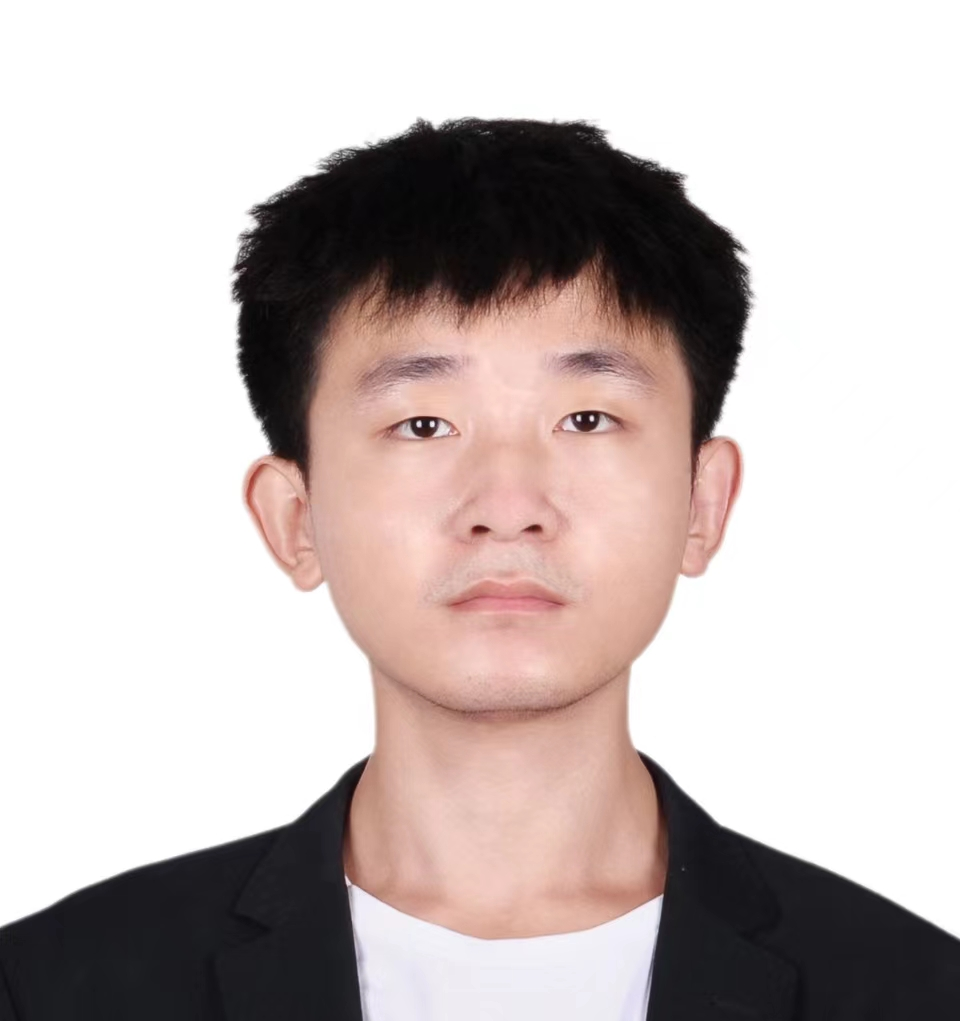
\includegraphics[width=1in,height=1.25in,clip,keepaspectratio]{zty}}]{Tingyu Zhang}
		Tingyu Zhang received the B.Sc. degree in Mathematics and Statistics from the Nanjing University of Information Science and Technology, Nanjing, China,
		in 2019. He is currently pursuing the Ph.D. degree
		in computer science and technology with Jilin University,
		Changchun. His current research interests
		include intelligent vehicles, point cloud analysis and 3D object detection.\end{IEEEbiography}
	\begin{IEEEbiography}[{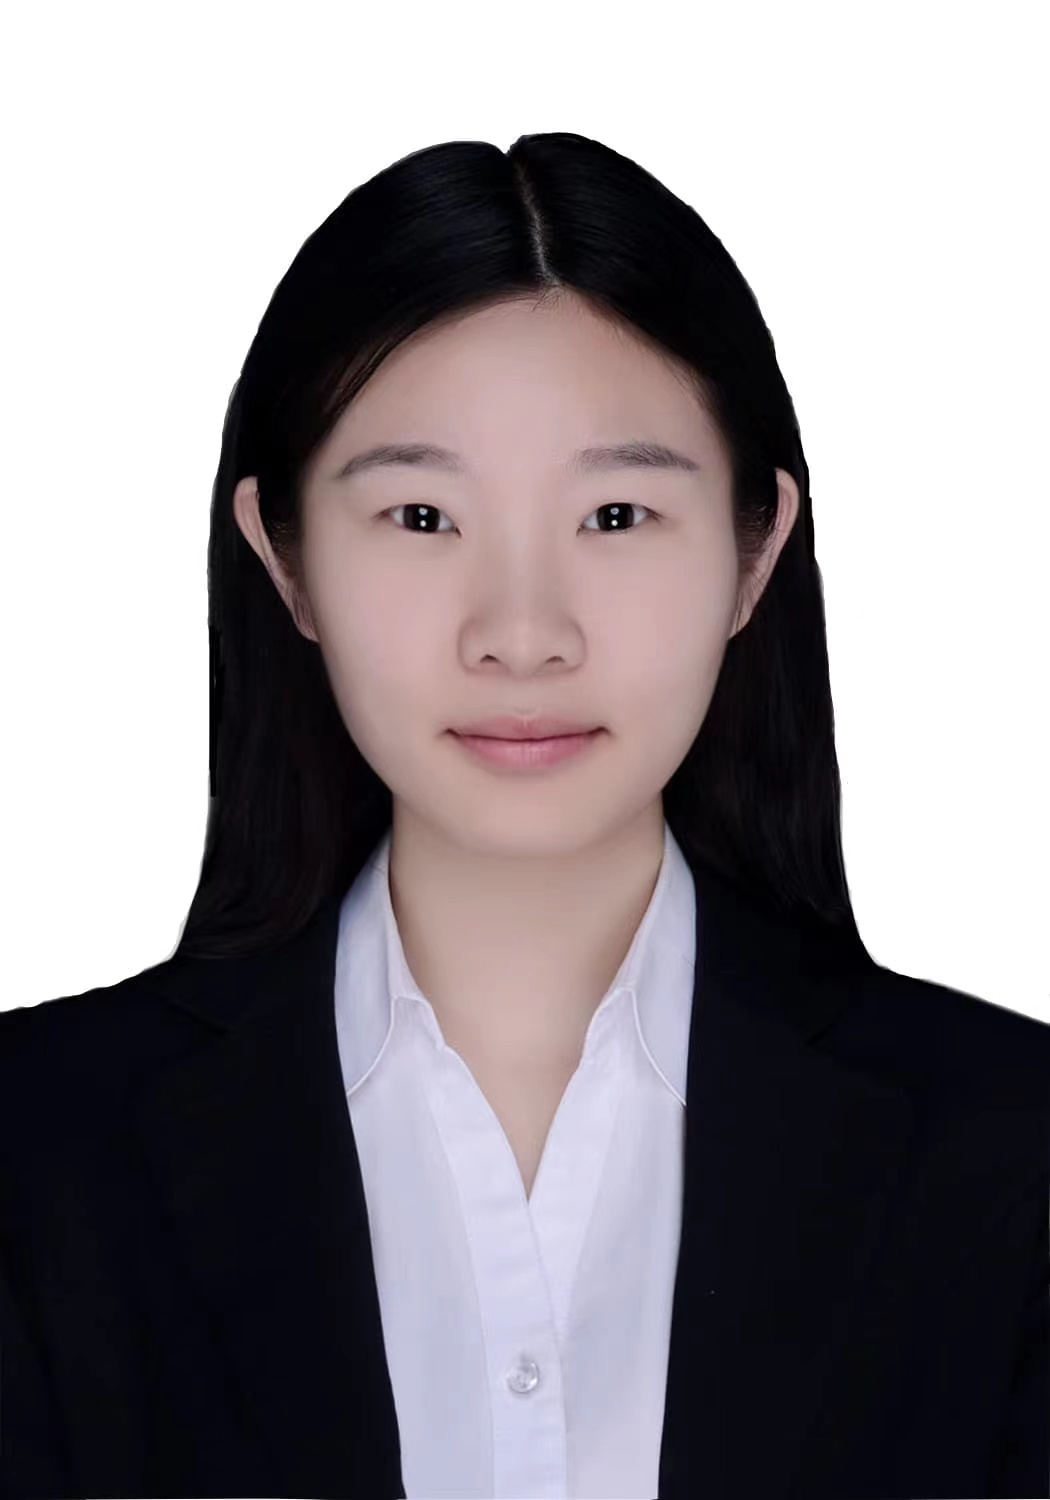
\includegraphics[width=1in,height=1.25in,clip,keepaspectratio]{yxy}}]{Xinyu Yang}
		Xinyu Yang received her master's degree in computer technique from Jilin University of science and technology. Her research interests include vehicular networks and intelligent driving, especially for privacy protection. She currently works for China Automotive Innovation Corporation.\end{IEEEbiography}
	
	
	
	\begin{IEEEbiography}[{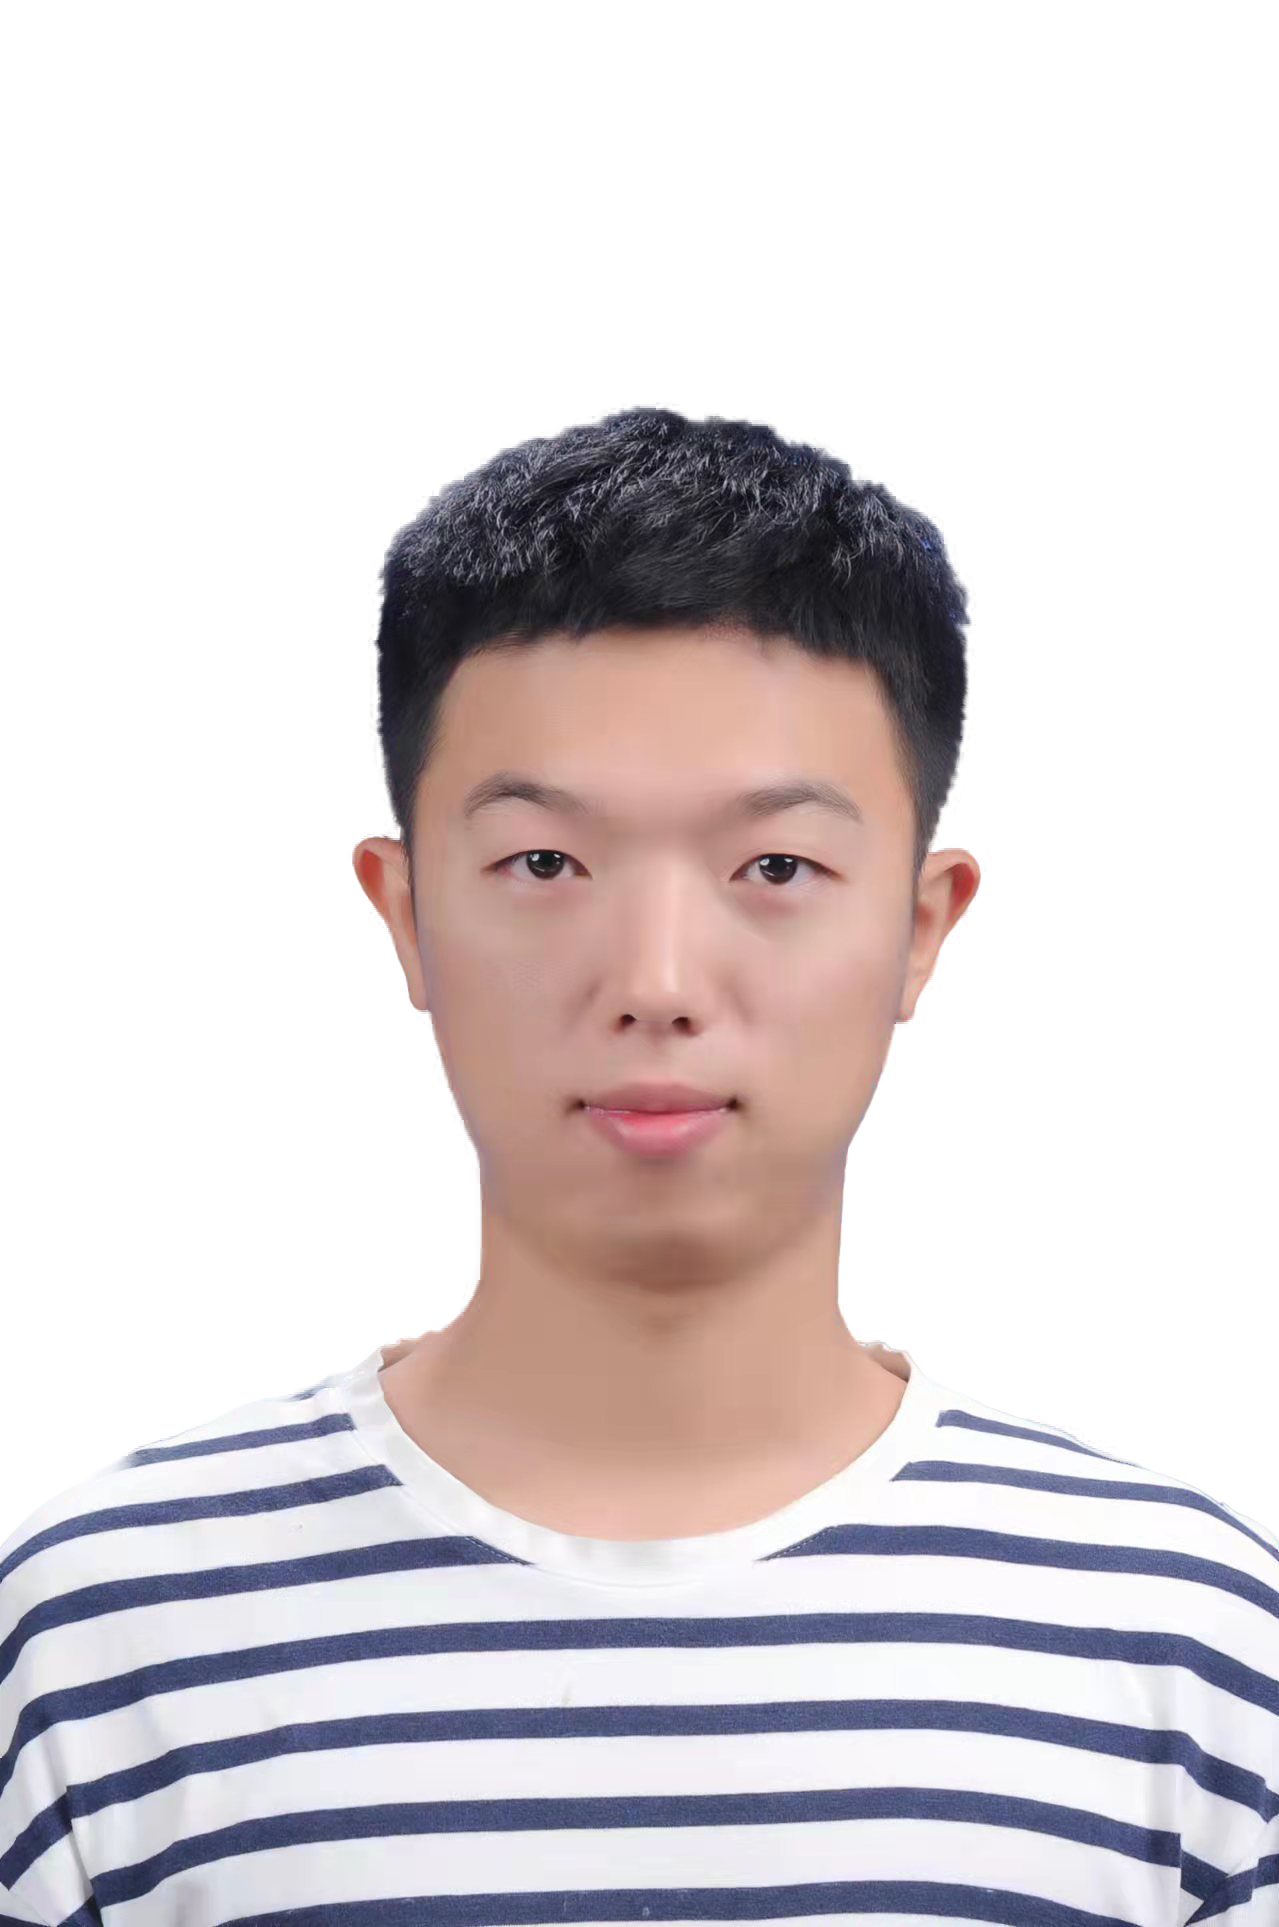
\includegraphics[width=1in,height=1.25in,clip,keepaspectratio]{lgz}}]{Zhigang Liang}
		Zhigang Liang graduated from Jilin University with a bachelor's degree in Engineering mechanics in 2019. He is currently pursuing a PhD in Computer Science and Technology at Jilin University in Changchun. His current research interests include self-driving car digital twin testing and intelligent transportation.\end{IEEEbiography}
	
	\begin{IEEEbiography}[{
\includegraphics[width=1in,height=1.25in,clip,keepaspectratio]{yyz}}]{Yanzhao Yang}
		Yanzhao Yang received his master's degree from Jilin University in 2011, major in Computer Science and Technology. He is currently pursuing the Ph.D degree in computer science and Technology with Jilin University, Changchun. His current research interests include intelligent vehicles, Physical Model of ADAS sensor and machine learning.\end{IEEEbiography}
	
	
	\begin{IEEEbiography}[{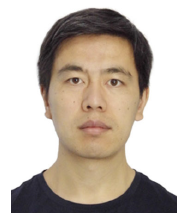
\includegraphics[width=1in,height=1.25in,clip,keepaspectratio]{wj}}]{Jian Wang}
		Jian Wang received the B.Sc., M.Sc., and Ph.D.
		degrees in computer science from Jilin University,
		Changchun, China, in 2004, 2007, and 2011, respectively.
		He is currently a Professor with the College of
		Computer Science and Technology, Jilin University.
		He has published over 60 articles in international
		journals. His research interests include wireless communication
		and vehicular networks, especially for
		network security and privacy protection.\end{IEEEbiography}
	
	
	
	
	
	
\end{document}


